\documentclass{article}



% --------------- PAQUETES ---------------
\usepackage[utf8]{inputenc}
\usepackage[spanish]{babel}
\usepackage{amsmath, amssymb}
\usepackage{physics}
\usepackage{xcolor}
\usepackage{tcolorbox}
\usepackage{cancel}
\usepackage{multicol}
\usepackage[
    top=2.5cm,
    bottom=2.5cm,
    left=3.3cm,
    right=3.3cm
]{geometry}
\usepackage{tikz}
\usetikzlibrary{angles, quotes}
\usepackage{float}

\definecolor{linkcolor}{HTML}{00a7d1}
\usepackage[colorlinks=true, allcolors=linkcolor]{hyperref}  


% --------------- COLORES PERSONALIZADOS ---------------
\definecolor{sectionColor}{HTML}{2240f0}
\definecolor{definicionColor}{HTML}{2240f0}
\definecolor{titleColor}{HTML}{ff0000}
\definecolor{exerciceColor}{HTML}{00d5ff}

% --------------- COMANDOS PERSONALIZADOS ---------------
\newcommand{\newsection}[1]{
    \vspace{0.5cm}
    {\color{sectionColor}
    \centering
    \section{\bl{#1}}}
    \color{black}
    \vspace{0.5cm}
}

\newcommand{\newsubsection}[1]{
    \vspace{0.5cm}
    \color{sectionColor}
    \subsection{ #1}
    \color{black}
    \vspace{0.5cm}
}

\newcommand{\newtitle}[1]{
    \color{titleColor}
    \subsubsection{\textbf{#1}}
    \color{black}
}

\newcommand{\newex}[1]{
    \vspace{0.5cm}
    \noindent{\large \color{exerciceColor} \textbf{#1}}\\[0.2cm]
}

\newcommand{\bl}[1]{\textbf{#1}}


\newtcolorbox{definicionbox}{
    colback=white,      % fondo blanco
    colframe=blue,     % borde negro
    boxrule=2pt,      % grosor del borde
    arc=0pt,            % sin esquinas redondeadas
    left=10pt, right=8pt, top=8pt, bottom=10pt, % margen interno
}

\newcommand{\definicion}[1]{%
    \vspace{0.5cm}
    \begin{definicionbox}
        #1
    \end{definicionbox}
    \vspace{0.5cm}
}

\newcommand{\ladoALado}[4]{
    \begin{minipage}[t]{#3\textwidth}
        \vspace{0pt}
        #1
    \end{minipage}
    \hfill
    \begin{minipage}[t]{#4\textwidth}
        \vspace{0pt}
        \centering
        \includegraphics[width=0.8\linewidth]{#2}
    \end{minipage}
}

% --------------- ENCABEZADO ---------------
\title{Apunte Física 1}
\author{Luca Di Bene}
\date{\today}

% --------------- DOCUMENTO ---------------
\begin{document}

    \maketitle
    \tableofcontents
    \newpage

% ------------------- SECCIÓN 1 -------------------
    \newsection{Unidades, Cantidades Físicas y Vectores}

    % ----------------- NUEVA SUBSECCIÓN -----------------

    \newsubsection{La Física}

    \par La Física es una \bl{ciencia experimental} que busca explicar fenómenos naturales a través de la observación y la experimentación. Los físicos formulan teorías mediante \bl{modelos ideales, leyes y principios físicos}. Estas teorías se desarrollan con creatividad, pruebas y observaciones, como hizo Galileo al investigar la caída de los cuerpos.

    \newtitle{Resolución de problemas}

    \par Resolver problemas permite aplicar conceptos. El proceso incluye:

    \begin{enumerate}
        \item \underline{Identificar conceptos}: Elegir qué principios físicos son relevantes.
        \item \underline{Plantear el problema}: Traducirlo a ecuaciones.
        \item \underline{Ejecutar la solución}: Sustituir valores y hacer cálculos.
        \item \underline{Evaluar la respuesta}: Verificar si tiene sentido físico.
    \end{enumerate} 

    \newtitle{Modelos idealizados}
    
    \begin{multicols}{2}

    \begin{center}
    \begin{minipage}[t]{0.60\textwidth}
    
        \smallskip

        \par En física, simplificamos los sistemas complejos creando \bl{modelos idealizados} que omiten detalles irrelevantes. Estos modelos son válidos dentro de ciertos límites, como el modelo de caída libre de Galileo que omite la resistencia del aire.
        \par La física describe el mundo mediante \bl{modelos matemáticos}, que permiten hacer predicciones razonables sobre el comportamiento de los sistemas.

    \end{minipage}

    \hfill
    \columnbreak
    
    \begin{minipage}[t]{0.25\textwidth}

        \bigskip
        \par Para simplificar el análisis de a) una pelota de béisbol lanzada al aire, usamos b) un modelo idealizado.
        \smallskip
        \par a) Una pelota real lanzada al aire.
        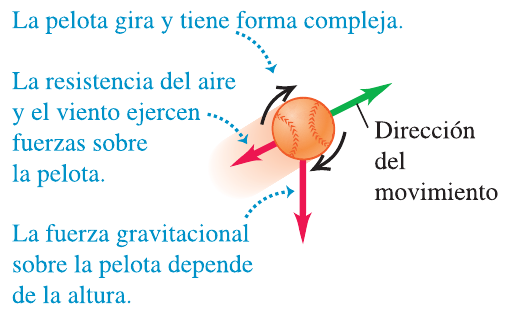
\includegraphics[width=\linewidth]{img/1.1-1.png}

        \par b) Un modelo idealizado de una pelota real lanzada al aire.
        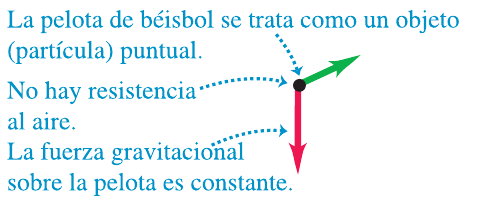
\includegraphics[width=\linewidth]{img/1.1-2.png}

    \end{minipage}
    \end{center}

    \end{multicols}

    % ----------------- NUEVA SUBSECCIÓN -----------------

    \newsubsection{Mediciones, magnitudes y unidades}

    \newtitle{Magnitudes físicas y unidades}

    \par Las \bl{magnitudes físicas} son propiedades medibles como masa, longitud o tiempo. El \bl{Sistema Internacional (SI)} define unidades básicas:

    \begin{itemize}
        \item \bl{Longitud}: metro (\bl{m})
        \item \bl{Masa}: kilogramo (\bl{kg})
        \item \bl{Tiempo}: segundo (\bl{s})
    \end{itemize}

    \par Las unidades derivadas (como velocidad o energía) se forman combinando unidades básicas.

    \newtitle{Conversión de unidades}

    \begin{enumerate}
        \item \underline{Identificar}: qué unidades hay que convertir.
        \item \underline{Plantear/Ejecutar}: usar factores de conversión.
        \item \underline{Evaluar}: comprobar que tenga sentido.
    \end{enumerate}

    \[
        3\cancel{\text{min}} \times \frac{60s}{1\cancel{\text{min}}} = 180s
    \]

    \newtitle{Incertidumbre}

    \par Toda medición tiene \bl{incertidumbre}, que refleja el límite del instrumento. Se expresa como:

    \[
        \text{valor medido} \pm \text{error}
    \]

% ------------------- NUEVA SUBSECCIÓN -------------------
    \newsubsection{Vectores y Suma de Vectores}

    \newtitle{Cantidades escalares y vectoriales}

    \par En física, algunas cantidades pueden ser descritas solo con un número y una unidad (\bl{escalares}), como el tiempo, la masa o la temperatura. Otras, en cambio, requieren una dirección además de una magnitud (\bl{vectores}). La velocidad y la fuerza son ejemplos típicos: no basta con saber cuánto valen, también es esencial saber \bl{hacia dónde} actúan o se mueven.
    \par Un vector se representa con una \bl{flecha}. La \bl{longitud} indica la magnitud y la \bl{orientación} muestra su dirección. Por convención, los vectores se nombran con letras negritas y con una \bl{flecha arriba}, como \(\vec{A}\), para diferenciarlos de los escalares.

    \begin{figure}[H]
        \centering
		\shorthandoff{>}
        \begin{tikzpicture}[scale=2]
            \draw[->] (0,0) -- (2,1) node[midway, above] {$\vec{A}$};
        \end{tikzpicture}
        \shorthandoff{>}
    \end{figure}

    \definicion{
        \centering
        \par \underline{Magnitud}: A o \(\lvert \vec{A} \rvert\) indican cuánto mide \(\vec{A}\), sin dirección.
        }

    \begin{multicols}{2}
        \centering

        \begin{minipage}[t]{0.6\textwidth}

            \par Dos vectores son \bl{iguales} si tienen la misma \bl{magnitud} y \bl{dirección}, aunque estén ubicados en lugares diferentes.

        \end{minipage}
        \hfill
        \columnbreak
        \begin{minipage}[t]{0.3\textwidth}

            \begin{figure}[H]
                \centering
				\shorthandoff{>}
                \begin{tikzpicture}[scale=1.2]
                    \draw[->, blue] (0,0) -- (1,1) node[midway, above] {$\vec{A}$};
                    \draw[->, red] (1,0) -- (2,1) node[midway, above] {$\vec{B}$};
                \end{tikzpicture}
                \shorthandoff{>}

            \end{figure}

        \end{minipage}
        
    \end{multicols}

    \begin{multicols}{2}
        \centering

        \begin{minipage}[t]{0.6\textwidth}

            \par Un vector \bl{opuesto} tiene igual magnitud pero direción contraria, lo llamamos el negativo del vector original.

        \end{minipage}
        \hfill
        \columnbreak
        \begin{minipage}[t]{0.3\textwidth}

            \begin{figure}[H]
                \centering
				\shorthandoff{>}
                \begin{tikzpicture}[scale=1.2]
                    \draw[->, blue] (0,0) -- (1,1) node[midway, above] {$\vec{A}$};
                    \draw[->, red] (2,1) -- (1,0) node[midway, below, right] {$\vec{B}=-\vec{A}$};
                \end{tikzpicture}
                \shorthandoff{>}

            \end{figure}

        \end{minipage}
        
    \end{multicols}

    \par \underline{Suma de vectores}: Para sumar vectores gráficamente, se usa el metodo "\bl{cola con punta}": se coloca el origen del segundo vector en el extremo del primero.
    \begin{figure}[H]
        \centering
		\shorthandoff{>}
        \begin{tikzpicture}[scale=1]
            \draw[->, gray] (0,0) -- (3,1) node[midway, below] {$\vec{A}$};
            \draw[->, gray] (3,1) -- (2,3) node[midway,right] {$\vec{B}$};
            \draw[->, blue] (0,0) -- (2,3) node[midway, above, left] {$\vec{A}+\vec{B}$};
        \end{tikzpicture}
        \shorthandoff{>}

    \end{figure}

    \par No importa el orden en que sumes los vectores, siempre da el mismo resultado.
    \[ \vec{A}+\vec{B}=\vec{B}+\vec{A} \]

    \par \underline{Resta de vectores}: Restar vectores significa sumar el \bl{opuesto}. Si queremos calcular \(\vec{A}-\vec{B}\), lo que realmente hacemos es sumar \(\vec{A}\) con el negativo de \(\vec{B}\).
    \[ \vec{A}-\vec{B}=\vec{A}+(-\vec{B}) \]

    % ---------------- NUEVA SUBSECCIÓN ----------------

    \newsubsection{Componentes de vectores}

    \par Cuando sumamos vectores, muchas veces es más fácil descomponerlos en \bl{componentes} sobre un sistema de ejes perpendiculares.
    \par Un vector \(\vec{A}\) puede descomponerse en dos vectores: uno paralelo al eje x (\(\vec{A}_x\)) y otro paralelo al eje y (\(\vec{A}_y\)). La suma de estos dos vectores da como resultado el vector original: \(\vec{A}=\vec{A}_x+\vec{A}_y\).

    \begin{figure}[H]
        \centering
		\shorthandoff{>}
        \begin{tikzpicture}[scale=1.2]
            \draw[->, black] (0,0) -- (3,0) node[below] {$x$};
            \draw[->, black] (0,0) -- (0,3) node[left] {$y$};

            \draw[->, blue] (0,0) -- (1,2) node[midway, above, left] {$\vec{A}$};
            \draw[->, red] (0,0) -- (1,0) node[midway, below] {$\vec{A}_x$};
            \draw[->, green] (0,0) -- (0,2) node[midway, above, left] {$\vec{A}_y$};
            \draw[-, dashed, gray] (1,0) -- (1,2);
            \draw[-, dashed, gray] (0,2) -- (1,2);

            % angle
            \draw[->, black] (0.5,0) .. controls (0.5,0.4) and (0.3,0.5) ..  (0.25,0.5) node[midway, above, right] {$\theta$};

        \end{tikzpicture}
		\shorthandoff{>}
    \end{figure}

    \par Podemos calcular la magnitud de las componentes de $\vec{A}$ si conocemos la magnitud A y su dirección. Describimos la direccion de un vector como el angulo $\theta$ formado por le eje x positivo con el vector en sentido anti horario. Entonces por definición de trigonométricas:
    \[ \lvert \vec{A}_x \rvert = \lvert \vec{A} \rvert \cos \theta \]
    \[ \lvert \vec{A}_y \rvert = \lvert \vec{A} \rvert \sin \theta \]

    \newsubsection{Vectores unitarios}

    \par Un \bl{vector unitario} es un vector con magnitud 1, sin unidades. Su única finalidad consiste en direccionar, es decir, describir una dirección en el espacio. En un sistema de coordenadas $x$-$y$ podemos definir un vector unitario $\hat{i}$ que apunte en la dirección del eje $+x$ y un vector unitario e $\hat{j}$ que apunte en la dirección del eje $+y$. Así, expresamos la relación entre vectores componentes y componentes, como sigue:

    \[ \vec{A}_x = A_x \hat{i} \]
    \[ \vec{A}_y = A_y \hat{j} \]

    Asimismo, escribimos un vector A en términos de sus vectores componentes como

    \[ \vec{A} = A_x \hat{i} + A_y \hat{j} \]

\newsection{Movimiento en dos o en tres dimensiones}

% ------------------- SECCIÓN 2 -------------------

\newsection{Leyes del movimiento de Newton}

\par En los dos capítulos anteriores estudiamos la cinemática, el lenguaje para describir el movimiento. Ahora estamos en condiciones de pensar en qué hace que los cuerpos se muevan como lo hacen.

\par En este capítulo usaremos dos conceptos nuevos, la fuerza y la masa, para analizar los principios de la dinámica, los cuales están establecidos en solo tres leyes que fueron claramente enunciadas por Sir Isaac Newton:

\begin{itemize}
    \item Primera ley (ley de la inercia): Si la fuerza neta sobre un cuerpo es cero, su movimiento no cambia.
    \item Segunda ley: Relaciona la fuerza con la aceleración cuando la fuerza neta no es cero.
    \item Tercera ley: Es una relación entre las fuerzas que ejercen dos cuerpos que interactúan entre sí.
\end{itemize}

\par Las leyes de Newton no son producto de deducciones matemáticas, sino una síntesis que los físicos han descubierto al realizar un sinnúmero de experimentos con cuerpos en movimiento.

    % ---------------- NUEVA SUBSECCIÓN ----------------

    \newsubsection{Fuerza e interacciones}

        \par En la vida cotidiana hablamos de fuerza como un empujón o un tirón. En física, una fuerza se define mejor como una interacción entre dos cuerpos o entre un cuerpo y su entorno. Esta interacción tiene dirección y magnitud, por lo que se representa como un vector.

    \newtitle{Fuerzas de contacto}

        \par Son fuerzas que requieren interacción directa entre cuerpos. Se distinguen principalmente tres tipos:

        \begin{itemize}
            \item \underline{Fuerza normal}: Es la fuerza ejercida por una superficie sobre un objeto en contacto con ella. Siempre actúa perpendicular a la superficie.
            \item \underline{Fuerza de fricción}: También es ejercida por una superficie, pero actúa paralela a ella y en dirección opuesta al movimiento relativo entre el objeto y la superficie.
            \item \underline{Fuerza de tensión}: Es la fuerza transmitida por cuerdas, cables o cordeles estirados. Actúa a lo largo del cordel y en la dirección de la tracción, como cuando se tira de una cuerda.
        \end{itemize}

        \begin{multicols}{3}
            \centering
            \begin{figure}[H]
                \centering
                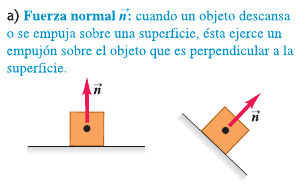
\includegraphics[scale=0.6]{img/2.1-1.png}
                \caption{Fuerza normal}
                \label{fig:Fuerza normal}
            \end{figure}

            \columnbreak

            \begin{figure}[H]
                \centering
                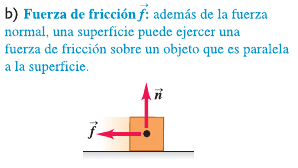
\includegraphics[scale=0.6]{img/2.1-2.png}
                \caption{Fuerza de fricción}
                \label{fig:Fuerza de fricción}
            \end{figure}

            \columnbreak

            \begin{figure}[H]
                \centering
                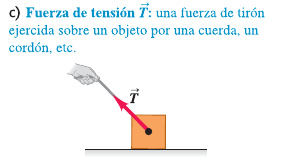
\includegraphics[scale=0.6]{img/2.1-3.png}
                \caption{Fuerza de tensión}
                \label{fig:Fuerza de tension}
            \end{figure}

        \end{multicols}

    \newtitle{Fuerzas a distancia}
        \par Estás actuar sin contacto física Ejemplos comunes son la gravedad, el magnetismo y las fuerzas eléctricas. La fuerza gravitatoria que la tierra ejerce sobre un objetto se llama \bl{peso}.
        \begin{figure}[H]
            \centering
            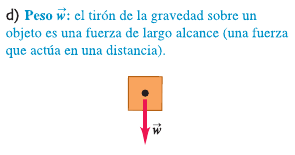
\includegraphics[scale=0.8]{img/2.1-4.png}
            \caption{Fuerza a distancia}
            \label{fig:Fuerza a distancia}
        \end{figure}

    \newtitle{Medición de fuerzas}

        \par La magnitud de una fuerza se mide en "newtons", que se abrevia N. (Daremos una definición precisa del newton más adelante) Un instrumento tipico para medirla es la \bl{balanza de resorte} que aprovecha la relación entre estiramento de un resorte y la fuerza aplicada.

    \newtitle{Superposición de fuerzas}

        \par Cuando varias fuerzas actúan sobre un cuerpo, su efecto combinado es igual al de una única fuerza resultante obtenida mediante la suma vectorial de todas ellas. Esto se conoce como el Principio de superposición. La fuerza neta o resultante total sobre un cuerpo es, la suma vectorial de todas las fuerzas que actúan sobre él. Se denota:
        
        \[\vec{R} = \sum \vec{F}\]

        \par Cada fuerza puede descomponerse en componentes vectoriales, entonces la fuerza neta tambien:

        \[\vec{R_x} = \sum \vec{F_x} \quad , \quad \vec{R_y} = \sum \vec{F_y}\]

    \newsubsection{Primera ley de Newton}

    \definicion{
        \par \color{blue}\underline{\bl{Primera ley}}\color{black}: Todo cuerpo persevera en su estado de reposo o movimiento uniforme y rectilíneo a no ser que sea obligado a cambiar su estado por fuerzas impresas sobre él. 
    }

    \par En esta ley se introduce el concerto de \bl{inercia}, que es la resistencia de un cuerpo a cambiar su estado de movimiento.
    \par Esta ley rompe con la idea aristotélica de que se necesita una fu constante para mantener el movimiento. Newton muestra que en r lo que se necesita es una fuerza para cambiar el movimiento.
    \par Si empujás una caja y después dejas de hacerlo, eventualmente se detiene. No porque "el movimiento se gasta", sino porque existen fuerzas Como la fricción y el rozamiento con el aire que actúan en sentido Contrario al movimiento y Provocan que se frene.

    \newtitle{Marcos de referencia inerciales}

    \par Un \bl{marco de referencia} es un sistema desde el cual se observa y describe el movimiento de los cuerpos.
    \par Un \bl{marco de referencia inercial} es aquel en el cual se cumple la Primera Ley de Newton, es decir que si un objeto cambia su Velocidad, entonces desde el marco se ve una fuerza actuando.

    \newsubsection{Segunda ley de Newton}

    \par Podemos ver que existe una relación proporcional entre la fuerza y la aceleración. Si empujamos una caja con una fuerza neta constante, la caja tendra una acelarión constante igual a $a=\vec{a}$.
    \par Si utilizamos una balanza de resorte Para aplicar una fuerza $\vec{F_1}$ obtenemos una aceleración $\vec{a}$, para $2\vec{F_1}$, obtenemos $2\vec{a}$ y para $\frac{1}{2}\vec{F_1}$ $\frac{1}{2}\vec{a}$. Muchos experimentos semejantes muestran que para un cuerpo dado, la magnitud de la aceleración es directamente propor-cional a la magnitud de la fuerza neta que actúa sobre él.

    \newtitle{Masa y fuerza}

   \par Nuestros resultados indican que para un cuerpo dado, el cociente $\left\lvert \Sigma \vec{F}\right\rvert $ entre $\left\lvert \vec{a} \right\rvert $ es constante. Llamamos a este cocient \bl{masa inercial} del cuerpo y la denotamos con \bl{m}. Es decir,

    \[ m = \frac{\lvert \Sigma \vec{F}\rvert }{\lvert \vec{a} \rvert } \quad,\quad
    \lvert \Sigma \vec{F} \rvert = m \lvert \vec{a} \rvert \quad o \quad
    \lvert \vec{a} \rvert = \frac{\lvert \Sigma \vec{F}\rvert }{m}\]

    \par La ultima de las ecuaciones indica que cuanto mayor sea su masa, más se "resiste" un cuerpo a ser acelerado.
    \par La unidad de masa en el SI es el kilogramo. Podemos usar este Kilogramo para definir el newton:

    \definicion{
        \par Un Newton es la cantidad de fuerza neta que proporciona una aceleración de 1 metro por segundo al cuadrado a un cuerpo con masa de 1 Kilograma.
    }

    \par Por la forma en que definimos el newton, está relacionado con las unidades de masa, longitud y tiempo.

    \[ 1 \text{N} = 1 \text{kg} \cdot \text{m/s}^2 \]

    \begin{table}[H]
        \centering
        \begin{tabular}{|c|c|c|c|}
            \hline
            Sistema de unidades & Fuerza & Masa & Aceleración \\
            \hline
            SI & Newton(N) & Kg & $m/s^2$ \\
            \hline
            cgs & dina(din) & g & $cm/s^2$ \\
            \hline
            Imperial & libra(lb) & slug & $ft/s^2$ \\
            \hline
        \end{tabular}
    \end{table}

    \newtitle{Enunciado de la segunda ley de Newton}

    \definicion{
        \par \color{blue}\underline{\bl{Segunda ley}}\color{black}: si una fuerza externa neta actúa sobre un Cuerpo, éste se acelera. La dirección de aceleración es la mis ma que la dirección de la fuerza neta. El vector de fuerza neta es igual a la masa del cuerpo multiplicada por su aceleración. En símbolos: 

        \[\Sigma \vec{F} = m \vec{a}\]
    }

    \par La segunda ley de Newton es una ley fundamental de la naturaleza, la relación básica entre fuerza y movimiento, Casa todo el resto del capítulo, y todo el que sigue, se dedica a aprender a aplicar este principio en diversas situaciones.

    \newtitle{Uso de la segunda ley de Newton}

    \par Hay al menos cuatro aspectos de la segundo ley de Newton que Merecen atención especial:

    \begin{enumerate}
        \item \bl{Forma de uso}: La segunda lev de Newton es una ecuación Vectorial, Pero normalmente se usa descompuesta por componentes:
        \[\Sigma \vec{F_x} = m \vec{a_x} \quad , \quad \Sigma \vec{F_y} = m \vec{a_y}\]

        \item \bl{Fuerzas externes}: La ley se refiere únicamente a Fuerzas externas es decir, ejercidas sobre el cuerpo desde otros cuerpos o el entorno. Un cuerpo no puede moverse por una fuerza que el mismo genera.
        \item \bl{Masa constante}: Estas ecuaciones solo son válidas si las masa no cambia. En casos donde la masa varía (cohete que pierda combustible) se necesita un tratamiento especial.
        \item \bl{Marcos de referencia inenciales}: La ley solo se aplica en marcos de referencia inerciales. No vale en marcos acelerados, como dentro de un auto que arranca.
    \end{enumerate}

    \newsubsection{Masa y Peso}

    \ladoALado{
        \par Es común usar incorrecta e indistintamente los términos \bl{masa} y \bl{peso} en las conversaciones cotidianas. Es absolutamente indispensable entender claramente las diferencias entre estas dos cantidades físicas.

        \par La \bl{masa} Caracteriza las Propiedades inerciales de un cuerpo. A mayor masa, se necesitará más fuerza Para causar una aceleración dada.

        \par El \bl{peso}, en cambio, es una fuerza ejercida sobre un cuerpo por la atracción de la Tierra.

        \par Para entender la relación entre masa y peso, note que un cuerpo en caída libre tiene una aceleración igual a gy, Por la segunda ley de Newton, una fuerza produce esa aceleración. Si un cuerpo de masam cae con una aceleración $\vec{g}$ con $ \lvert \vec{g} \rvert = 9.8 \text{m/s}^2 $, entonces: $\vec{w} = m \vec{g}$
    }{img/2.4-1.png}{0.7}{0.3}

    \newtitle{Variación de g con la ubicación}

    \par En la tierra se usa $g \approx 9,80 m/s^2$, Pero varía entre $9,78$ y $9,82 m/s^2$. Esa variación se debe a la forma de la tierra y su rotación. El peso cambia con g, Pero la masa no.

    \vspace{3cm}

    \newtitle{Medición de masa y peso}

    \par En la práctica, se mide la masa de un cuerpo midiendo su peso y Comparándolo con un estandar. Por la ecuación $w=mg$, si dos cuerpos tienen el mismo peso en el mismo lugar, entonces tienen la misma masa.

    \newsubsection{Tercera ley de Newton}

    \par No podemos tirar de una perilla sin que ésta tire de nosotros. Al Patear un balón de fútbol, la fuerza hacia adelante que el rie ejerce sobre él lo lanza en su trayectoria, pero sentimos la fuerza que el balón ejerce sobre el pie.
    \par Los experimentos muestran que, al interactuar dos cuerpos, las fuer-zas que ejercen mutuamente son iguales en magnitud y opuestas en dire-ceión. Ésta es la tercera ley de Newton.

    \definicion{
        \par \color{blue}\underline{\bl{Tercera ley}}\color{black}: si el cuerpo A eserce una fuerza sobre el cuerpo. B ("\text{acción}"), entonces, B ejerce una fuerza sobre A ("\text{reacción}"). Estas dos fuerzas tienen la misma magnitud Pero dirección opuesta, y actúan sobre diferentes cuerpos.
        \[\vec{F}_{AB} = - \vec{F}_{BA}\]
    }

    \begin{figure}[H]
        \centering
        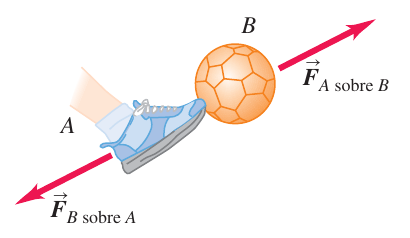
\includegraphics[scale=0.8]{img/2.5-1.png}
    \end{figure}

    \par Expresando en palabras, en la tercera ley de Newton, "acción" y "reacción" son las dos fuerzas opuestas, y Podemos llamarlas \bl{Par acción-reacción}.

    \newsubsection{Diagramas de cuerpo libre}

    \par En esta sección mencionaremos algunas ideas y técnicas que Pueden usarse en cualquier problema en que intervengan las leves de Newton.

    \begin{enumerate}
        \item Las leves de Newton se aplican a un cuerpo específico. Siempre tenés que definir que cuerpo vas a analizar.
        \item En la sumatoria de fuerzas F, solo se incluyen las fuerzas que actúan sobre el cuerpo, no las que el cuerpo ejerce sobre otros. Si analizás a una persona caminando, incluís la fuerzas del suelo sobre la persona, no la que la persona ejerce sobre el suelo.
        \item Un diagrama de cuerpo libre muestra el cuerpo aislado con todas las fuerzas externas que actúan sobre el, sin incluir fuerzas que el cuerpo ejerce sobre otros.
    \end{enumerate}

    \begin{figure}[H]
        \centering
        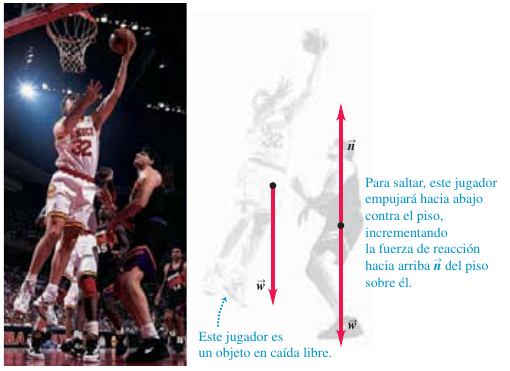
\includegraphics[scale=0.7]{img/2.6-1.png}
    \end{figure}

\newsection{Aplicación de las leyes de Newton}

\par Este capítulo se enfoca en \bl{aplicar las leyes de Newton} a distintos tipos de situaciones reales, como un velero deslizándose sobre hielo, un trineo bajando una colina y un avión dando una vuelta cerrada. A pesar de que las \bl{leyes de Newton} son simples en su formulación, resolver problemas concretos requiere una buena dosis de análisis y técnica.

    \newsubsection{Empleo de la primera ley de Newton: Partículas en equilibrio}

    \par El principio físico fundamental es la primera ley de Newton: si una partícula está en reposo o se mueve con velocidad constante en un marco de referencia inercial, la fuerza neta que actúa sobre ella, es decir, la suma vectorial de todas las fuerzas que actúan sobre ella debe ser cero:

    \definicion{
        \centering
        \par $\Sigma \vec{F} = 0 \quad$ (partícula en equilibrio, forma vectorial)
    }

    \par Esta sección trata sobre el uso de la primera ley de Newton para resolver problemas de cuerpos en equilibrio. Quizás algunos de los problemas parezcan complicados; no obstante, lo importante es recordar que todos los problemas que implican partículas en equilibrio se resuelven igual.

    \newex{Ejercicio 1. Equilibrio unidimensional: Tensión en una cuerda sin masa}

    \par Una gimnasta de masa $m_G = 50.0 kg$ se cuelga del extremo inferior de una cuerda colgante. El extremo superior está fijo al techo de un gimnasio. Suponga que la masa de la cuerda es despreciable.
    \begin{enumerate}
        \item ¿Cuánto pesa la gimnasta?
        \item ¿Qué fuerza (magnitud y dirección) ejerce la cuerda sobre ella?
        \item ¿Qué tensión hay en la parte superior de la cuerda?
    \end{enumerate}
    
    \newex{Solución 1.}

    \par Primero identificamos que la gimnasta y la cuerda, ambos estan en equilibrio. Tenemos como incognita el peso de la gimnasta $w_G$. La cuerda tira de la gimnasta con una fuerza $T_{CG}$ y la gimnasta tira de la cuerda con una fuerza $T_{GC}$. El techo ejerce otra fuerza sobre la cuerda, $T_{TC}$, que provoca que la cuerda y la gimnasta esten en equilibrio.

    \begin{figure}[H]
        \centering
        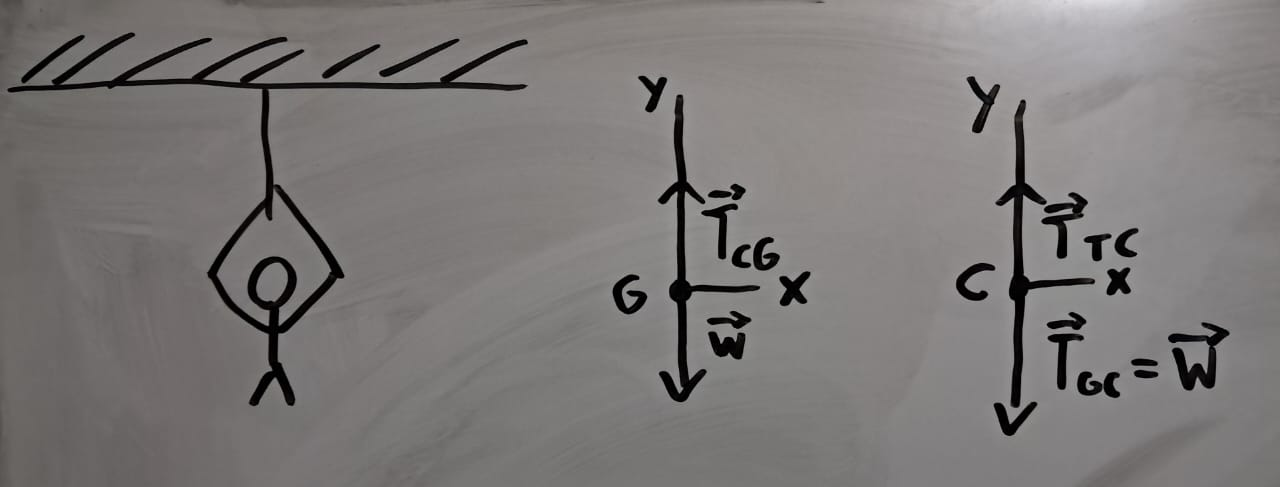
\includegraphics[width=\textwidth]{img/3.1-1.png}
    \end{figure}

    \par El primer digrama representa la situación en si. El segundo diagrama representa las fuerzas que actúan sobre la gimnasta. El tercer diagrama representa las fuerzas que actúan sobre la cuerda.

    \quad

    \par Para calcular el peso de la gimnasta ($\vec{w}$), usaremos la ecuación de la gravedad, derivada de la segunda ley de Newton:

    \[ \lvert \vec{w} \rvert = m \cdot 9.8 \text{m/s}^2 \]
    \[ w_G = 50 \text{kg} \cdot 9.8 \text{m/s}^2 \]
    \[ w_G = 490 \text{N} \]

    \begin{center}
        \par \bl{El peso de la gimnasta es de 490 Newtons}.
    \end{center}

    \par Entonce la magnitud de la fuerza que ejerce la cuerda sobre la gimnasta es: $T_{CG} = 490 \text{N}$. Y su dirección es contraria a la del peso de la gimnasta.

    \par Por el par acción-reacción, existe la fuerza $\vec{T}_{GC} = - \vec{T}_{CG} = \vec{w}$, entonces la gimnasta tira de la cuerda con una fuerza de 490 Newtons con una dirección que apunta hacia abajo. Entonces la fuerza $\vec{T}_{TC}$ es igual en magnitud a $\vec{T}_{GC}$ pero con dirección opuesta, es decir, $\vec{T}_{TC} = - \vec{T}_{GC}$.

    \quad

    \par La \bl{tensión de la cuerda} es de $T_{TC} = 490 \text{N}$ en la parte superior de la cuerda y de $T_{CG} = 490 \text{N}$ en la parte inferior de la cuerda.

    \newsubsection{Empleo de la segunda ley de Newton: Dinámica de partículas}

    \par Ahora podemos analizar problemas de dinámica, donde aplicamos la segunda ley de Newton a cuerpos sobre los cuales la fuerza neta no es cero, de manera que los cuerpos no están en equilibrio sino que tienen aceleración.

    \definicion{
        \centering
        \( \Sigma \vec{F} = m \vec{a} \)
    }

    \newex{Ejercicio 2. Movimiento rectilíneo con una fuerza constante}

    \par Un velero para hielo descansa en una superficie horizontal sin fricción (figura 5.7a). Sopla un viento constante (en la dirección de los patines del trineo), de modo que 4.0 s después de soltarse el velero adquiere una velocidad de 6.0 m>s (unos 22 km/h o 13 mi/h). ¿Qué fuerza constante $F_w$ ejerce el viento sobre el velero? La masa total del velero más el tripulante es de 200 kg.

    \newex{Solución 2.}

    \par Identificamos las variables que se nos dan:

    \begin{itemize}
        \item $m = 200 \text{kg}$
        \item $v(0s) = 0.0 \text{m/s}$
        \item $v(4s) = 22.0 \text{km/h} = 6.1 \text{m/s}$
    \end{itemize}

    \par Para calcular la fuerza usaremos la segunda ley de Newton: $\Sigma \vec{F} = m \vec{a}$. Pero primero debemos calcular la aceleración. Como tenemos una velocidad incial y otra 4s despues podemos utilizar:
    \[ a = \frac{v_1 - v_0}{t_1 - t_0} \]

    \[ a = \frac{6.1 \text{m/s} - 0.0 \text{m/s}}{4.0 \text{s}} = 1.525 \text{m/s}^2 \]

    \par Por lo tanto, la fuerza constante que ejerce el viento sobre el velero es de $F_w = 200 \text{kg} \cdot 1.525 \text{m/s}^2 = 305 \text{N}$

    \newtitle{Peso aparente e ingravidez aparente}

    \par Cuando un pasajero de masa m viaja en un elevador con aceleración ay , una báscula da como peso aparente del pasajero:

    \[ w = m \cdot (g + a_y) \]

    \par Cuando el elevador está acelerando hacia arriba, $a_y$ es positiva y $n$ es mayor que el peso del pasajero $w = mg$. Si el elevador acelera hacia abajo, ay es negativa y n es menor que el peso. Si el pasajero no sabe que el elevador está acelerando, sentirá que su peso cambia y, de hecho, la báscula lo indica. El caso extremo sucede cuando el elevador tiene una aceleración hacia abajo $a_y = -g$, es decir, cuando está en caída libre. En este caso, $n = 0$ y el pasajero siente que no tiene peso.

    \newex{Ejercicio 3. Aceleración cuesta abajo}

    \par Un trineo cargado de estudiantes en vacaciones (peso total $w$) se desliza hacia abajo por una larga cuesta nevada. La pendiente tiene un ángulo constante $\alpha$, y el trineo está tan bien encerado que la fricción es despreciable. ¿Qué aceleración tiene el trineo?

    \newex{Solución 3.}

    \par Necesitamos averiguar la aceleración $a$. Sabemos que la unica fuerza que actua sobre el trineo es la gravedad, y que su peso es $w$.

    \par Para mayor comodidad dibujaremos un diagrama de cuerpo libre inclinado para que el eje x se paralelo a la aceleración $a$, ahora $a_x$.

    \begin{figure}[H]
        \centering
        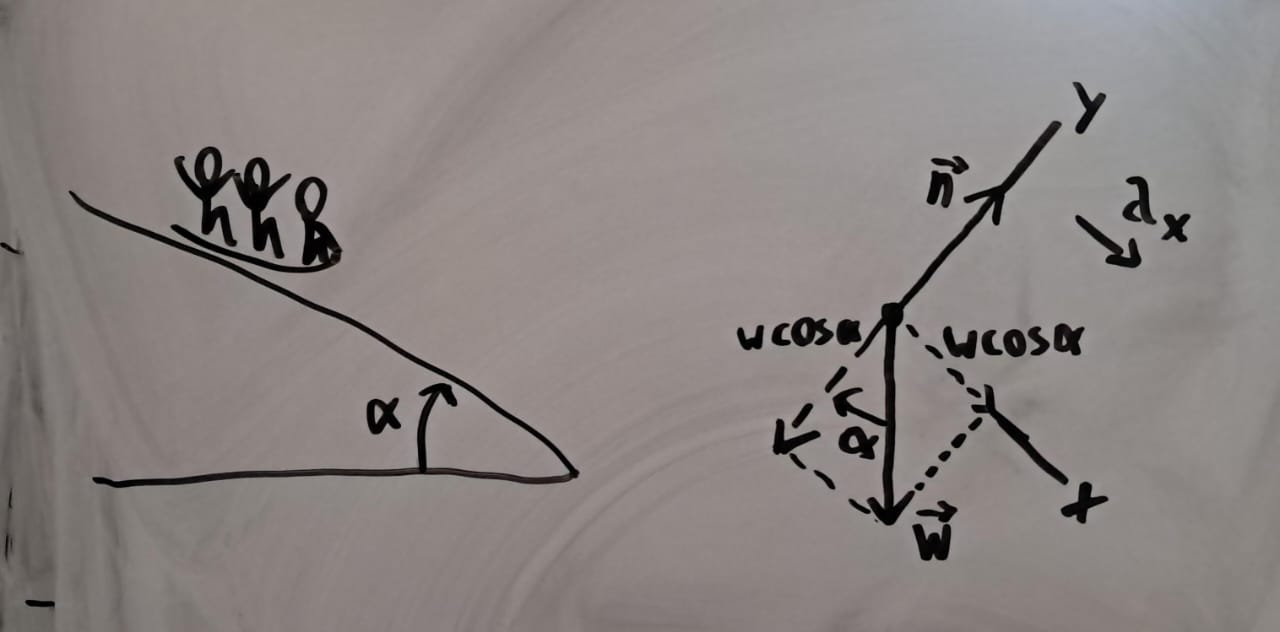
\includegraphics[width=\textwidth]{img/3.2-2.png}
    \end{figure}

    \par Por segunda ley de Newton dividida en componentes tenemos:

    \[ \Sigma F_x = m a_x \]

    \[ \Sigma F_y = m a_y \]

    \par Si sumamos las fuerzas:

    \[ \Sigma F_y = w\cos(\alpha) + (-w\cos(\alpha)) = 0 = m a_y \quad \Longrightarrow  \quad a_y = 0 \]

    \[ \Sigma F_x = w\sin(\alpha) = m a_x \]

    \par Como $w = m g$, tenemos que $\cancel{m} a_x = \cancel{m} g \sin(\alpha)$, dejando como resultado:

    \[ a_x = g \sin(\alpha) \]

    \newsubsection{Fuerzas de fricción}

    \par Hemos visto varios problemas en que un cuerpo descansa o se desliza sobre una superficie que ejerce fuerzas sobre el cuerpo. En esta sección, veremos con detenimiento la fuerza de fricción.

    \par Una fuerza importante en muchos aspectos de nuestra vida es la fricción. El aceite de un motor automotriz reduce la fricción entre piezas móviles; no obstante, sin fricción entre los neumáticos y el asfalto, el automóvil no podría avanzar ni dar vuelta.

    \vspace{7cm}

    \newtitle{Fricción cinética y estática}

    \ladoALado{
        \par Primero, cuando un cuerpo descansa o se desliza sobre una superficie, podemos representar la fuerza de contacto que la superficie ejerce sobre el cuerpo en términos de componentes de fuerza perpendiculares y paralelos a la superficie (figura). El vector componente paralelo a la superficie (y perpendicualr a n ) es la fuerza de fricción, denotada con $\vec{f}$. La dirección de la fuerza de fricción siempre es opuesta al movimiento relativo de las dos superficies.
    }{img/3.3-1.png}{0.6}{0.4}

    \par El tipo de fricción que actúa cuando un cuerpo se desliza sobre una superficie es la \bl{fuerza de fricción cinética $\vec{f}_k$}. La magnitud de esta fuerza suele aumentar al aumentar la fuerza normal. En muchos casos, la magnitud de la fuerza de fricción cinética $f_k$ experimental es aproximadamente proporcional a la magnitud n de la fuerza normal. En tales casos, representamos la relación con la ecuación:

    \definicion{
        \centering
        \par \( f_k = \mu_k \cdot n \) \quad \quad \quad (magnitud de la fuerza de fricción cinética)
    }

    \par donde $\mu_k$ es una constante llamada coeficiente de fricción cinética. Cuanto más resbalosa sea una superficie, menor será el coeficiente de fricción. Al ser el cociente de dos magnitudes de fuerza ($\frac{{f}_k}{{n}}$), $\mu_k$ es un número puro sin unidades. (Caso similar a la masa inercial).

    \vspace{0.5cm}

    \par \color{red} \underline{DISCLAIMER}: \color{black} La ecuación sólo es una representación aproximada de un fenómeno complejo. En el nivel microscópico, las fuerzas de fricción y la normal se deben a las fuerzas intermoleculares (fundamentalmente eléctricas) entre dos superficies ásperas en los puntos donde entran en contacto.

    \vspace{0.5cm}

    \par Las fuerzas de fricción también pueden actuar cuando no hay movimiento relativo. Si tratamos de deslizar por el piso una caja con libros, tal vez no se mueva porque el piso ejerce una fuerza de fricción igual y opuesta sobre la caja. Ésta se llama \bl{fuerza de fricción estática $\vec{f}_s$}.

    \begin{figure}[H]
        \centering
        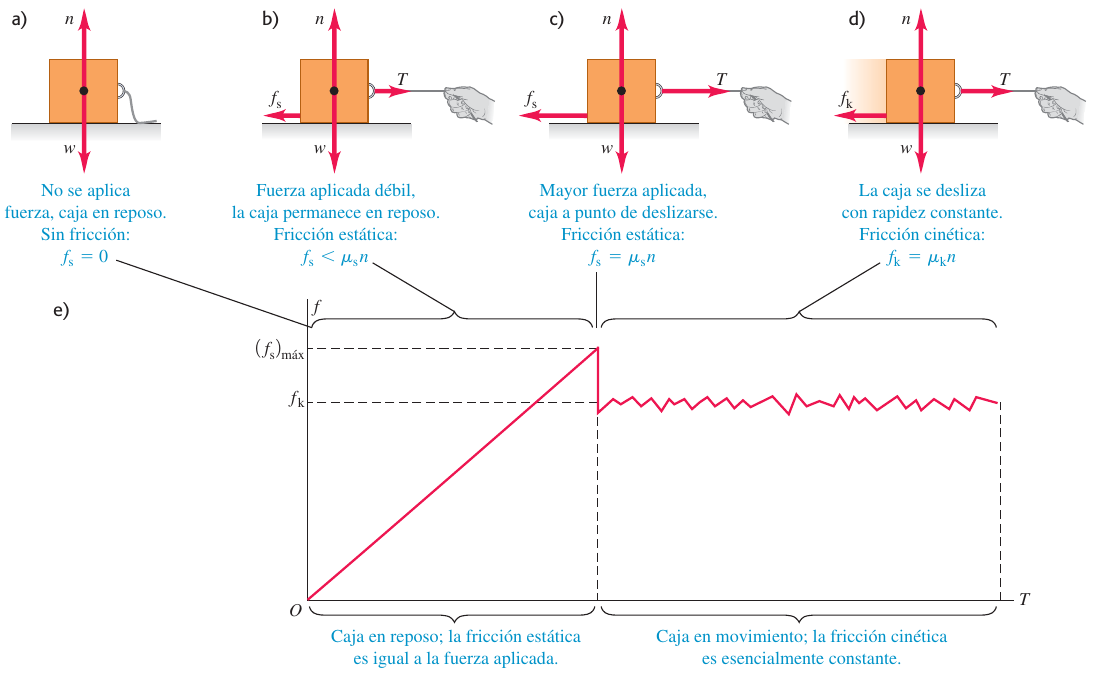
\includegraphics[width=\textwidth]{img/3.3-2.png}
    \end{figure}

    \begin{center}
        \par \bl{Tabla: Coeficientes de fricción aproximados}
    \end{center}

    \begin{table}[H]
        \centering
        \begin{tabular}{|c|c|c|}
            \hline
            Materiales & Coeficiente de fricción estática, $\mu_s$ & Coeficiente de fricción cinética, $\mu_k$ \\
            \hline
            Acero sobre acero & 0.74 &  0.57 \\
            \hline
            Aluminio sobre acero & 0.61 &  0.47 \\
            \hline
            Cobre sobre acero & 0.53 &  0.36 \\
            \hline
            Latón sobre acero & 0.51 &  0.44 \\
            \hline
            Zinc sobre hierro colado & 0.85 &  0.21  \\
            \hline
            Cobre sobre hierro colado & 1.05 &  0.29  \\
            \hline
            Vidrio sobre vidrio & 0.94 &  0.40  \\
            \hline
            Cobre sobre vidrio & 0.68  &  0.53  \\
            \hline
            Teflón sobre teflón & 0.04 &  0.04 \\
            \hline
            Teflón sobre acero & 0.04 &  0.04 \\
            \hline
        \end{tabular}
    \end{table}

    \newex{Ejercicio 4. Fricción en movimiento horizontal}

    \par Usted intenta mover una caja de $500N$ por un piso horizontal. Para comenzar a moverla, debe tirar con una fuerza horizontal de $230N$. Una vez que la caja “se libera” y comienza a moverse, puede mantenerse a velocidad constante con sólo $200N$. ¿Cuáles son los coeficientes de fricción estática y cinética?

    \newex{Solución 4.}

    \par Sabemos que la caja esta en reposo cuando se le aplica una fuerza de $230N$ en el eje x.

    \begin{figure}[H]
        \centering
        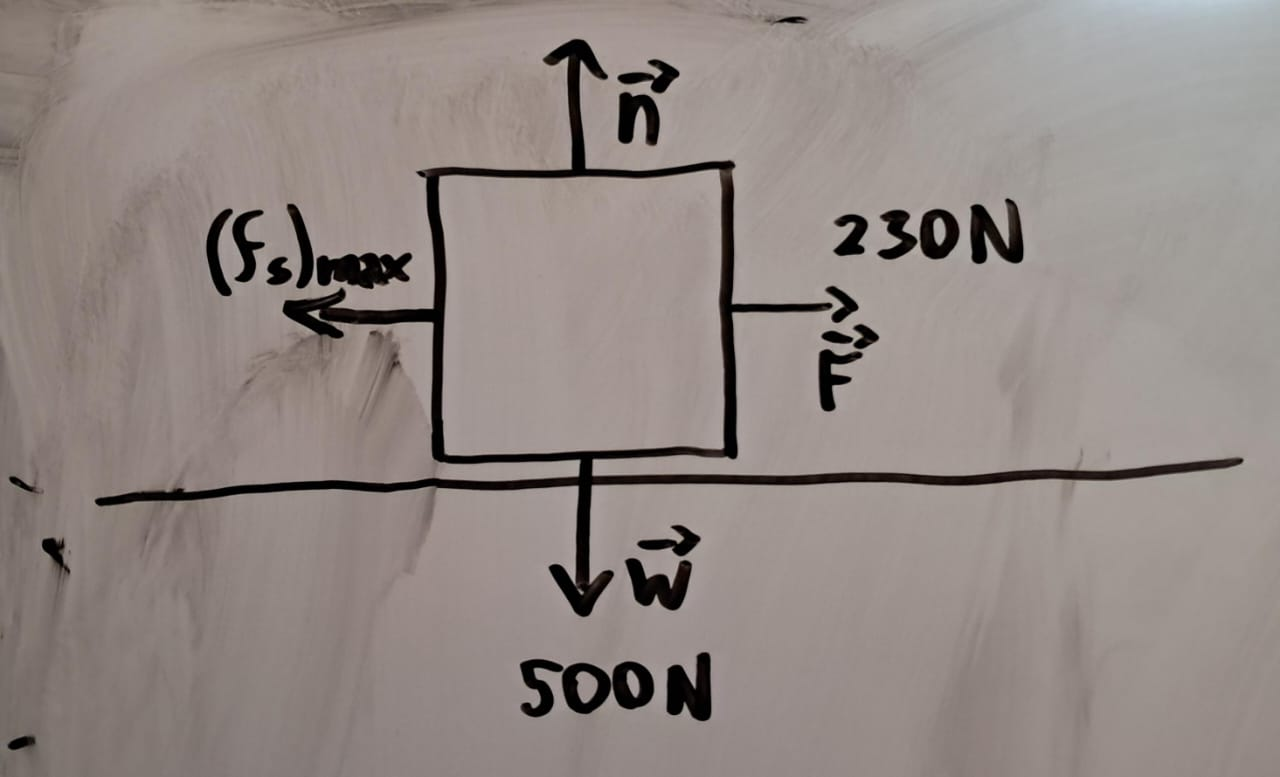
\includegraphics[width=0.5\textwidth]{img/3.3-3.png}
    \end{figure}

    \par Usando la primera ley de Newton por componentes tenemos:

    \[ \Sigma F_x = n + (-w) = 0 \quad \Longrightarrow \quad n = w = 500N \]

    \[ \Sigma F_y = F + (-(f_s)_{max}) = 0 \quad \Longrightarrow \quad F = (f_s)_{max} = 230N \]

    \par Entonces podemos calcular el coeficiente de fricción estática:

    \[ \mu_s = \frac{F}{n} = \frac{230N}{500N} = 0.46 \]

    \par También sabemos que si la caja esta en movimiento horizontal se mantendra en equilibrio si se le aplica una fuerza de $200N$:

    \begin{figure}[H]
        \centering
        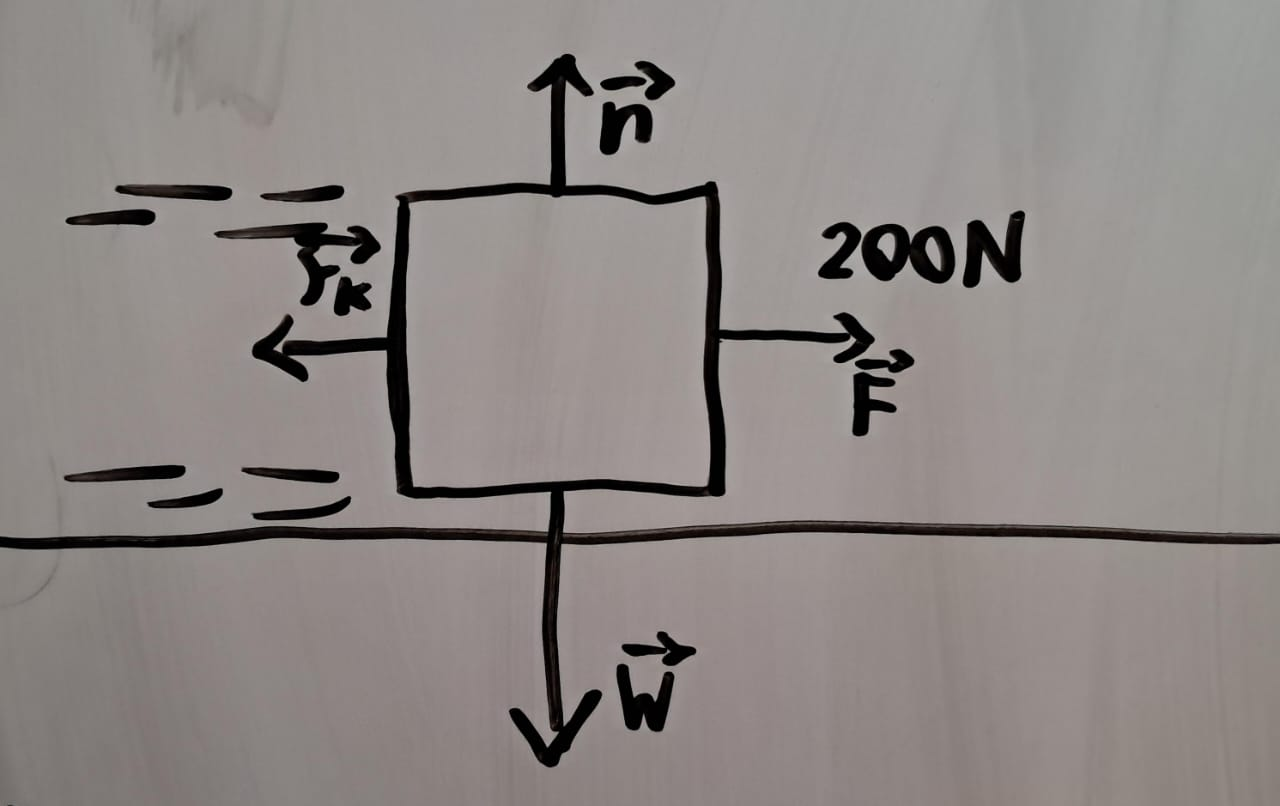
\includegraphics[width=0.5\textwidth]{img/3.3-4.png}
    \end{figure}

    \par Usando la primera ley de Newton por componentes tenemos:

    \[ \Sigma F_x = n + (-w) = 0 \quad \Longrightarrow \quad n = w = 500N \]

    \[ \Sigma F_y = F + (-f_k) = 0 \quad \Longrightarrow \quad F = f_k = 200N \]

    \par Entonces podemos calcular el coeficiente de fricción cinética:

    \[ \mu_k = \frac{F}{n} = \frac{200N}{500N} = 0.4 \]

    \par Concluimos que el coeficiente de fricción estática es $0.46$ y el coeficiente de fricción cinética es $0.4$.

    \newex{Ejercicio 5. Reducción al mínimo de la fricción cinética}

    \par En el ejercicio anterior, suponga que usted intenta mover la caja atando una cuerda a ella y tira de la cuerda hacia arriba con un ángulo de 30° sobre la horizontal. ¿Qué fuerza debe aplicar al tirar para mantener la caja en movimiento con velocidad constante? ¿Esto es más fácil o difícil que tirar horizontalmente? Suponga que $w = 500N$ y $\mu_k = 0.40$.

    \newex{Solución 5.}

    \par Sabemos que la caja esta en equilibrio (su velocidad es constante) entonces aplicamos la primera ley de Newton para encontrar la fuerza $T$ que se debe aplicar para mantener la caja en movimiento:

    \par Primero hacemos un diagrama de cuerpo libre:

    \begin{figure}[H]
        \centering
        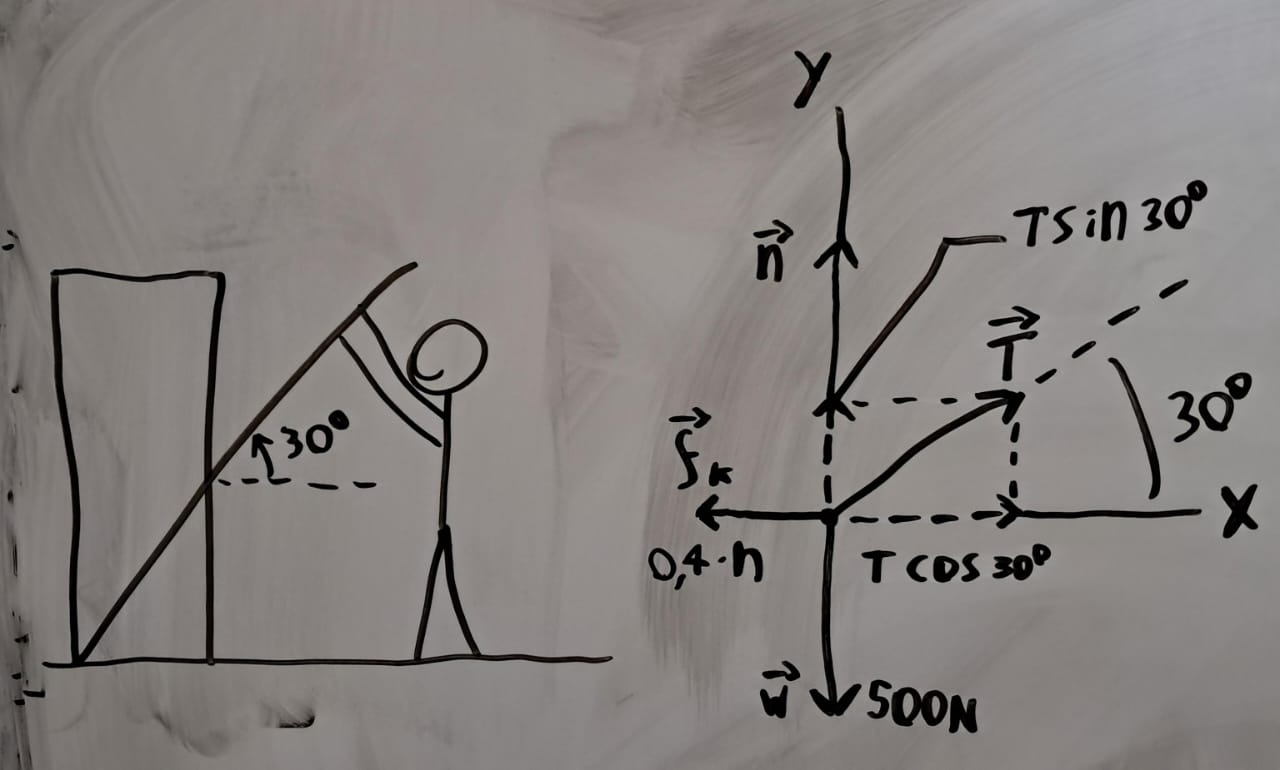
\includegraphics[width=0.8\textwidth]{img/3.3-5.png}
    \end{figure}

    \par Usando la primera ley de Newton por componentes tenemos:

    \[ \Sigma F_x = T\cos(30^\circ) + (-f_k) = 0 \quad \Longrightarrow \quad T\cos(30^\circ) = f_k \]

    \[ \Sigma F_y = T\sin(30^\circ) + n + (-w) = 0 \quad \Longrightarrow \quad n = w - T\sin(30^\circ) \]

    \vspace{0.5cm}

    \par Para encontrar la fuerza $T$ tenemos que usar el hecho de que $f_k = T\cos(30^\circ)$:

    \[ T\cos(30^\circ) = f_k = \mu_k \cdot n \]

    \par Remplazando:

    \[ T\cos(30^\circ) = \mu_k \cdot (w - T\sin(30^\circ)) \]

    \par Despejando $T$ tenemos:

    \[ T = \frac{\mu_k \cdot w}{cos(30^\circ) + \mu_k \sin(30^\circ)} = \frac{0.40 \cdot 500N}{cos(30^\circ) + 0.40 \sin(30^\circ)} \approx 188N \]

    \vspace{0.5cm}

    \par Concluimos que la fuerza $T$ que debe aplicar para mantener la caja en movimiento es de 188N.

    \vspace{0.5cm}

    \par Por otro lado, si se intenta mover la caja horizontalmente, entonces la fuerza $T$ que se debe aplicar para mantener la caja en movimiento es de $\mu_k \cdot n = 0.40 \cdot 500N = 200N$. Al no ser reducida la fuerza normal $f_k$ no se reduce por lo que la fricción "jode" más al tratar de mover la caja.

    \newtitle{Fricción de rodamiento}

    \par Es mucho más fácil mover un archivero lleno de documentos sobre un piso horizontal usando un carrito con ruedas que deslizándolo. Podemos definir un \bl{coeficiente de fricción de rodamiento $\mu_r$}, que es la fuerza horizontal necesaria para lograr rapidez constante en una superficie plana, dividida entre la fuerza normal hacia arriba ejercida por la superficie. Cuyo valor suele ser de 0.002 a 0.003 para ruedas de acero sobre rieles de acero, y de 0.01 a 0.02 para ruedas de caucho sobre concreto.

    \newex{Ejercicio 6. Movimiento con fricción de rodamiento}

    \par ...

    \newtitle{Resistencia de fluidos y rapidez terminal}

    \par Si usted saca la mano por la ventanilla de un automóvil que viaja con gran rapidez, comprobará la existencia de la \bl{resistencia de un fluido}, que es la fuerza que un fluido (gas o líquido) ejerce sobre un cuerpo que se mueve a través de él.

    \par La dirección de la fuerza de resistencia de un fluido que actúa sobre un cuerpo siempre es opuesta a la dirección de la velocidad del cuerpo. La magnitud de la fuerza de resistencia de un fluido suele aumentar al incrementarse la rapidez del cuerpo en el fluido. Esto es muy diferente de la fuerza de fricción cinética entre dos superficies en contacto, que casi siempre podemos considerar independiente de la rapidez. A rapidez baja, la magnitud f de la fuerza de resistencia del fluido es aproximadamente proporcional a la rapidez $v$ del cuerpo:

    \definicion{ 
        \centering
        $f = k v$ \quad \quad (resistencia del fluido a baja rapidez)
        }

    
    \noindent donde $k$ es una constante de proporcionalidad que depende de la forma y el tamaño del cuerpo, y las propiedades del fluido. Las unidades de este $k$ son $ [k] = \frac{N}{m/s} = \frac{kg \cdot \frac{m}{s^2} \cdot s }{m} = \frac{kg}{s}$.

    \par La fuerza de resistencia es aproximadamente proporcional a $v^2$, no a $v$, para la rapidez de una pelota de tenis o una rapidez mayor y se denomina \bl{arrastre del aire} o sólo arrastre. En este caso, sustituimos la ecuación por la siguiente:

    \definicion{
        \centering
        $f = D v^2$ \quad \quad (resistencia de fluidos a alta rapidez)
    }

    \par Por la dependencia de $v^2$, el arrastre aumenta rápidamente conforme se incrementa la rapidez. Las unidades de este $D$ son $ [D] = \frac{N}{m^2/s^2} = \frac{kg \cdot \frac{m}{s^2} \cdot s^2 }{m^2} = \frac{kg}{m}$.

    \vspace{0.5cm}

    \par Por los efectos de la resistencia de fluidos, un objeto que cae en un fluido no tiene aceleración constante. Para describir su movimiento debemos partir de la segunda ley de Newton.

    \vspace{2cm}

    \ladoALado{
        \par Consideremos esta situación: suponga que usted suelta una roca en la superficie de un estanque profundo, y cae hasta el fondo (figura). En este caso, la fuerza de resistencia del fluido está dada por la ecuación de resistencia del fluido a baja rapidez. ¿Cómo cambian la aceleración, velocidad y posición de la roca con el tiempo?
    }{img/3.3-6.png}{0.6}{0.4}

    \par Si observamos el diagrama de cuerpo libre podemos ver que $\Sigma F_x = 0$ entonces solo tomamos en cuenta la componente $y$:

    \[ \Sigma F_y = mg + (-f) = mg + (-kv_y) = ma_y \]

    \par Al principio, cuando la roca empieza a moverse, $v_y = 0$, la fuerza de resistencia es cero y la aceleración inicial es $a_y = g$. Al aumentar la rapidez, también se incrementa la fuerza de resistencia hasta ser igual en magnitud al peso. Ahora, $mg - kv_y = 0$, la aceleración se vuelve cero y ya no aumenta la rapidez. A esta rapidez final $v_t$, se le llama \bl{rapidez terminal}, y esta dada por $mg - kv_t = 0$, es decir:

    \[ v_t = \frac{mg}{k} \quad \quad \text{(\bl{rapidez terminal})} \]

    \par La siguiente figura muestra cómo varían la aceleración, la velocidad y la posición con el tiempo.

    \begin{figure}[H]
        \centering
        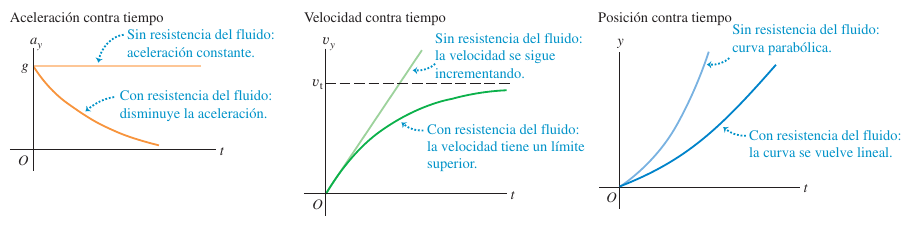
\includegraphics[width=\textwidth]{img/3.3-7.png}
    \end{figure}

    \newsubsection{Dinámica del movimiento circular}

    \par Cuando una partícula se mueve en un círculo con rapidez constante, su aceleración siempre es hacia el centro del círculo (perpendicular a la velocidad instantánea). La magnitud $a_{rad}$ de la aceleración es constante y está dada en términos de la rapidez $v$ y el radio $R$ del círculo por

    \definicion{
        \centering
        \( a_{rad} = \frac{v^2}{R} \) \quad \quad (movimiento circular uniforme)
    }

    \par El subíndice “$rad$” nos recuerda que en cada punto la aceleración siempre es radial hacia el centro del círculo, perpendicular a la velocidad instantánea. Se le denomina \bl{aceleración centrípeta}.

    \vspace{0.5cm}

    \ladoALado{
        \par El movimiento circular uniforme, como todos los movimientos de una partícula, se rige por la segunda ley de Newton. Para hacer que la partícula acelere hacia el centro del círculo, la fuerza neta $\Sigma \vec{F}$ sobre la partícula debe estar dirigida siempre hacia el centro. La magnitud de la aceleración es constante, así que la magnitud $F_{net}$ de la fuerza neta también debe ser constante. Si deja de actuar la fuerza neta hacia adentro, la partícula saldrá disparada en una línea recta tangente al círculo (ver figura).
    }{img/3.3-8.png}{0.6}{0.4}

    \par ...


    \newsubsection{Fuerzas fundamentales de la naturaleza}

    \par Hemos visto fuerzas de varios tipos —peso, tensión, fricción, resistencia de fluidos y la fuerza normal— y veremos otras más al seguir estudiando física. Pero, ¿cuántas clases distintas de fuerzas hay? Actualmente, se considera que todas las fuerzas son expresiones de tan sólo cuatro clases de fuerzas o interacciones fundamentales entre las partículas.
    
    \ladoALado{
        \par Las \bl{interacciones gravitacionales} incluyen la fuerza familiar del peso, que se debe a la acción de la atracción gravitacional terrestre sobre un cuerpo. La mutua atracción gravitacional entre las diferentes partes de la Tierra mantienen a nuestro planeta unido (figura a).

        \vspace{0.2cm}

        \par Las \bl{interacciones electromagnéticas}, incluye las fuerzas eléctricas y magnéticas. Si nos frotamos un peine por el cabello, al final el peine tendrá una carga eléctrica; es posible usar la fuerza eléctrica para atraer trocitos de papel. Todos los átomos contienen carga eléctrica positiva y negativa, así que átomos y moléculas pueden ejercer fuerzas eléctricas unos sobre otros (figura b).

        \vspace{0.2cm}

        \par Las otras dos clases de interacciones son menos conocidas. La \bl{interacción fuerte} mantiene unido el núcleo de un átomo. Los núcleos contienen neutrones (eléctricamente neutros) y protones (con carga positiva). La fuerza eléctrica entre protones hace que se repelan mutuamente; la enorme fuerza de atracción entre las partículas nucleares contrarresta esta repulsión y mantiene el núcleo estable. En este contexto, la interacción fuerte también se denomina fuerza nuclear fuerte; tiene un alcance mucho menor que las interacciones eléctricas, pero es mucho más fuerte dentro de ese alcance. La interacción fuerte juega un papel fundamental en las reacciones termonucleares que ocurren en el núcleo del Sol, y que generan el calor y su luz (figura c).

        \vspace{0.2cm}

        
    }{img/3.3-9.png}{0.6}{0.33}
    \par Por último, tenemos la \bl{interacción débil} cuyo alcance es tan pequeño que es relevante sólo a una escala de núcleo o menor. La interacción débil causa una forma común de radioactividad, llamada desintegración beta, en la que un neutrón de un núcleo radioactivo se transforma en protón al tiempo que expulsa un electrón y una partícula casi sin masa llamada antineutrino electrónico. La interacción débil entre un antineutrino y la materia ordinaria es tan tenue que el antineutrino fácilmente podría atravesar una pared de plomo ¡de un millón de kilómetros de espesor! Incluso cuando una estrella gigante sufrió una explosión cataclísmica llamada supernova, la mayoría de la energía fue liberada mediante la interacción débil (figura d).

    \vspace{2cm}

    \newsection{Trabajo y Energía Cinética}

    \par En este capítulo nos concentraremos en la mecánica. Conoceremos una importante forma de energía, la energía cinética o la energía de movimiento, y su relación con el concepto de trabajo. También consideraremos la potencia, que es la rapidez con que se realiza trabajo.

    \newsubsection{Trabajo}

    \par En esta sección aprenderemos cómo se define el trabajo y cómo se calcula en diversas situaciones que implican fuerzas constantes. Aunque ya sabemos cómo resolver problemas donde las fuerzas son constantes, el concepto de trabajo nos resultará útil. Más adelante en este capítulo deduciremos la relación entre trabajo y energía cinética, y la aplicaremos después en problemas donde las fuerzas no son constantes.

    \par Estos tres ejemplos de trabajo —mover un sofá, levantar una pila libros y empujar un automóvil— tienen algo en común. En ellos realizamos trabajo ejerciendo una fuerza sobre un cuerpo mientras éste se mueve de un lugar a otro, es decir, sufre un desplazamiento. Efectuamos más trabajo si la fuerza es mayor (empujamos más fuerte el auto) o si el desplazamiento es mayor (lo empujamos una mayor distancia).

    \par El físico define el trabajo con base en estas observaciones. Considere un cuerpo que sufre un desplazamiento de magnitud $s$ en línea recta. (Por ahora, supondremos que todo cuerpo puede tratarse como partícula y despreciaremos cualquier rotación o cambio en la forma del cuerpo.) Mientras el cuerpo se mueve, una fuerza constante $\vec{F}$ actúa sobre él en la dirección del desplazamiento $\vec{s}$. Definimos el trabajo $W$ realizado por esta fuerza constante en dichas condiciones como el producto de la magnitud $F$ de la fuerza y la magnitud $s$ del desplazamiento:

    \definicion{
        \centering
        \(W = Fs\) \text{(fuerza constante en dirección del desplazamiento rectilíneo)}
    }

    \par La unidad de trabajo en el SI es el joule (que se abrevia $J$ y se pronuncia “yul”,nombrada así en honor del físico inglés del siglo XIX James Prescott Joule). En el SI la unidad de fuerza es el newton y la unidad de distancia es el metro, así que 1 joule equivale a un new-ton-metro ($N \cdot m$):

    \[1 J = 1 N \cdot m\]

    \par En el sistema británico, la unidad de fuerza es la libra (Ib), la unidad de distancia es el pie (ft), y la unidad de trabajo es el pie-libra ($ft \cdot Ib$). Estas conversiones son útiles:

    \[1 J =  0.7376 ft \cdot 1Ib \quad \quad  1 ft \cdot lb = 1.356 J\]

    \vspace{0.5cm}

    \par Pensemos en una persona que empuja un automóvil averiado. Si lo empuja a lo largo de un desplazamiento $\vec{s}$ con una fuerza constante $\vec{F}$ en la dirección del movimiento, la cantidad de trabajo que efectúa sobre el auto está dada por la ecuación:$W = Fs$. Sin embargo, ¿y si la persona hubiera empujado con un ángulo $\phi$ con respecto al desplazamiento del auto (figura)?

    \begin{figure}[H]
        \centering
        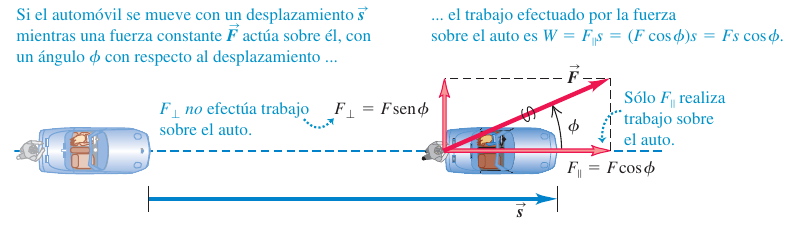
\includegraphics[width=\textwidth]{img/5.1-1.png}
        
    \end{figure}
    
    \par Entonces $\vec{F}$ tiene una componente $F_{\parallel} = F cos \phi$ en la dirección del desplazamiento y una componente $F_{\perp} = F sin \phi$ que actúa perpendicular al desplazamiento.

    \par En este caso, sólo la componente paralela $F_{\parallel}$ es eficaz para mover el auto, por lo que definimos el trabajo como el producto de esta componente de fuerza y la magnitud del desplazamiento. Por lo tanto:

    \[W = Fs cos \phi \]

    \par La ecuación tiene la forma del producto escalar de dos vectores. Ello nos permite escribir la ecuación de forma más compacta:

    \[W = \vec{F} \cdot \vec{s}\]

    \newex{Ejercicio 7. Trabajo efectuado por una fuerza constante}

    \par a) Esteban ejerce una fuerza constante de magnitud $210N$ sobre el automóvil averiado de la figura anterior, mientras lo empuja una distancia de $18m$. Además, un neumático se desinfló, así que, para lograr que el auto avance al frente, Esteban debe empujarlo con un ángulo de $30^\circ$ con respecto a la dirección del movimiento. ¿Cuánto trabajo efectúa Esteban?

    \par b) Con ánimo de ayudar, Esteban empuja un segundo automóvil averiado con una fuerza constante $\vec{F} = (160N)\hat{i} - (40N)\hat{j}$. El desplazamiento del automóvil es $\vec{s} = (14m)\hat{i} + (11m)\hat{j}$ ¿Cuánto trabajo efectúa Esteban en este caso?

    \newex{Solución 7.}

    \par ...

    \newtitle{Trabajo: Positivo, negativo o cero}

    \par En el ejercicio anterior, el trabajo efectuado al empujar los autos fue positivo. No obstante, es importante entender que el trabajo también puede ser negativo o cero. Ésta es la diferencia esencial entre la definición de trabajo en física y la definición “cotidiana” del mismo.

    \begin{figure}[H]
        \centering
        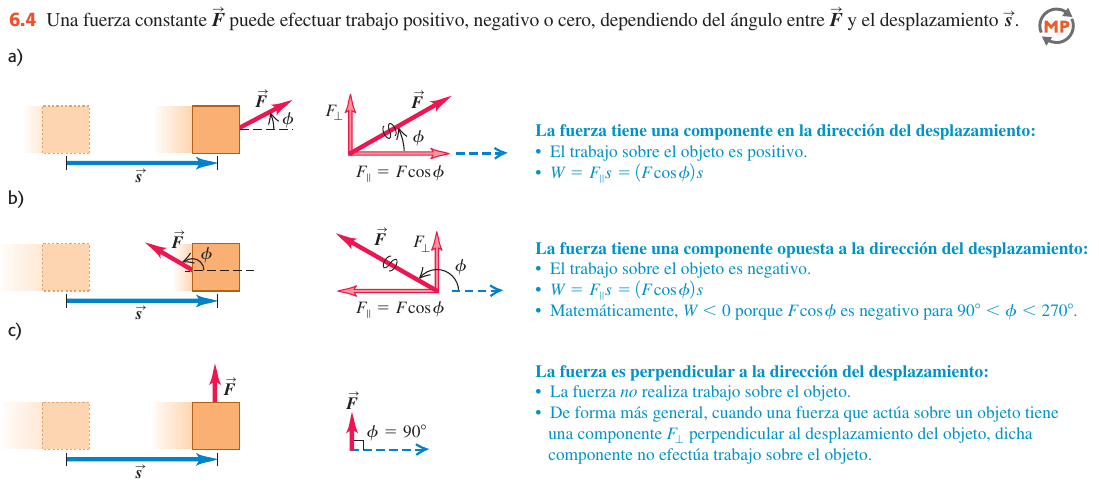
\includegraphics[width=\textwidth]{img/5.1-2.png}
    \end{figure}

    \newtitle{Trabajo total}

    \par ¿Cómo calculamos el trabajo cuando varias fuerzas actúan sobre un cuerpo? Podemos usar las ecuaciones anteriormente vistas para calcular el trabajo realizado por cada fuerza individual. Puesto que el trabajo es una cantidad escalar, el trabajo total $W_{tot}$ realizado por todas las fuerzas sobre el cuerpo es la suma algebraica de los trabajos realizados por las fuerzas individuales. Otra forma de calcular $W_{tot}$ es calcular la suma vectorial de las fuerzas (es decir, la fuerza neta) y usarla en vez de $\vec{F}$.

    \newex{Ejercicio 8. Trabajo realizado por varias fuerzas}

    \par Un granjero engancha su tractor a un trineo cargado con leña y lo arrastra 20 m sobre el suelo horizontal. El peso total del trineo y la carga es de $14700 N$. El tractor ejerce una fuerza constante de $5000 N$ a $36.9^\circ$ sobre la horizontal. Una fuerza de fricción de $3500 N$ se opone al movimiento del trineo. Calcule el trabajo realizado por cada fuerza que actúa sobre el trineo y el trabajo total de todas las fuerzas.

    \newex{Solución 8.}

    \begin{figure}[H]
        \centering
        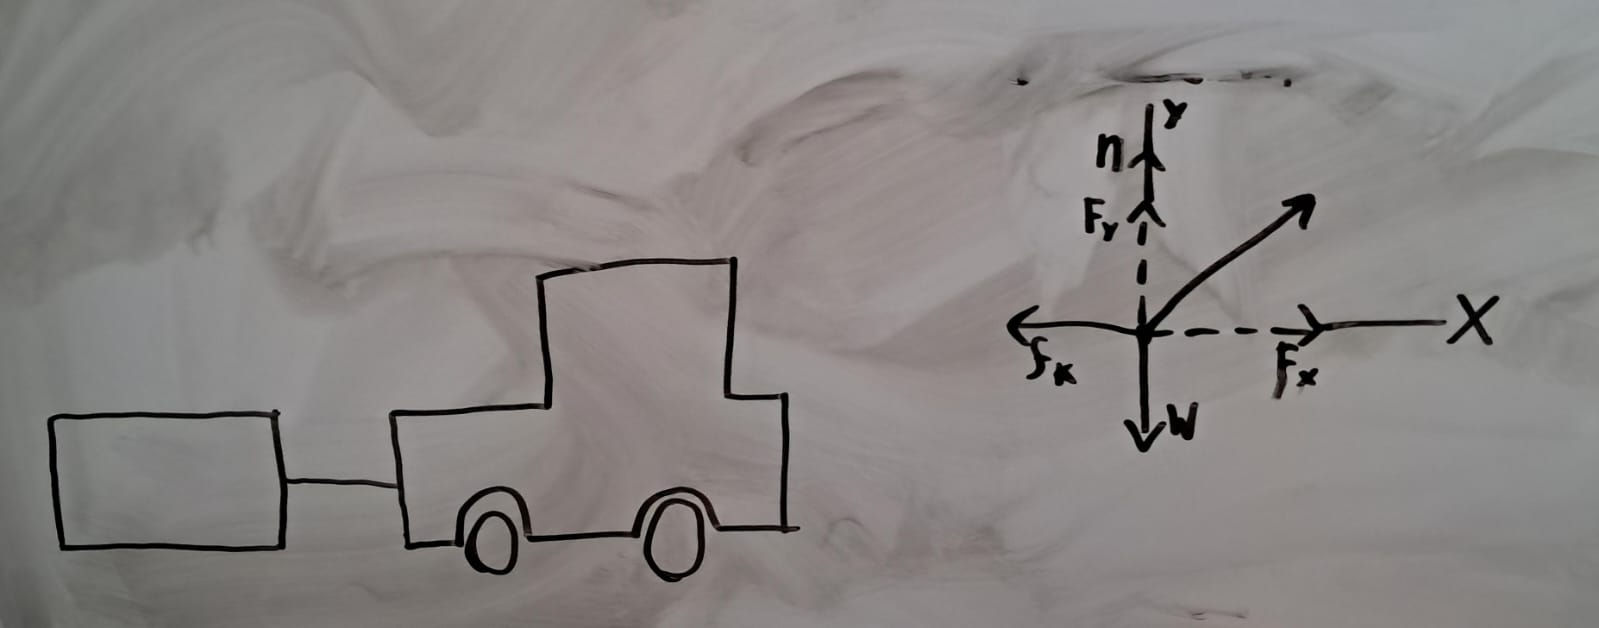
\includegraphics[width=\textwidth]{img/5.1-3.png}
    \end{figure}

    \par ...
    
    \vspace{6cm}

    \newsubsection{Energía cinética y el teorema trabajo-energía}

    \par El trabajo total realizado por fuerzas externas sobre un cuerpo se relaciona con el desplazamiento de éste (los cambios en su posición), pero también está relacionado con los cambios en la rapidez del cuerpo. Para comprobarlo, considere la siguiente figura, que muestra tres ejemplos de un bloque que se desliza sobre una mesa sin fricción. Las fuerzas que actúan sobre el bloque son su peso $\vec{w}$, la fuerza normal $\vec{n}$ y la fuerza $\vec{F}$ ejercida por la mano.

    \begin{figure}[H]
        \centering
        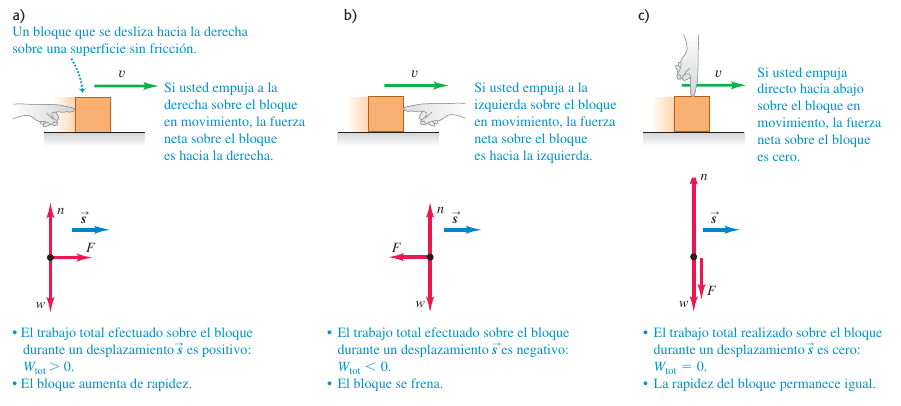
\includegraphics[width=\textwidth]{img/5.2-1.png}
    \end{figure}
    
    \par Hagamos más cuantitativas tales observaciones. Considere una partícula con masa $m$ que se mueve en el eje $x$ bajo la acción de una fuerza neta constante de magnitud $F$ dirigida hacia el eje $+x$ (figura). La aceleración de la partícula es constante y está dada por la segunda ley de Newton, $F = m a_x$. Suponga que la rapidez cambia de $v_1$ a $v_2$ mientras la partícula sufre un desplazamiento $s = x_2 - x_1$ del punto $x_1$ al $x_2$.

    \begin{figure}[H]
        \centering
        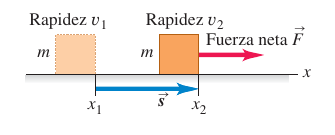
\includegraphics[width=0.5\textwidth]{img/5.2-2.png}
    \end{figure}

    \par Primero buscamos una ecuación que solo relaciona $v$, $a_x$ y $s$ (el desplazamiento). Para ello utilizamos estas ecuaciones de MRUA:

    \[\text{1.}\quad v = v_1 + a_xt\]

    \[\text{1.}\quad x = x_1 + v_1t + \frac{1}{2}a_xt^2\]

    \par Eliminamos el tiempo $t$ (utilizando 1.):

    \[t = \frac{v-v_1}{a_x}\]

    \par Sustituyendo en la ecuación de posición:

    \[s = x - x_1 = v_1 t + \frac{1}{2} a_x t^2\]

    \[s = v_1 \left(\frac{v-v_1}{a_x}\right)  + \frac{1}{2} a_x \left(\frac{v-v_1}{a_x}\right) ^2\]

    \par Multiplicamos y simplificamos:

    \[s = \frac{v_1 (v - v_1)}{a_x} + \frac{(v-v_1)^2}{2 a_x}\]

    \par Multiplicamos todo por $2a_x$

    \[ 2a_x s = 2 v_1 (v - v_1) + (v - v_1)^2 \]

    \par Expandimos:

    \[ 2a_x s = 2 v_1 v - 2 v_1^2 + v^2 - 2 v_1 v + v_1^2\]

    \par Se cancelan los términos $2v_1v - 2v_1v$, y queda:

    \[ 2a_x s = v^2 - v_1^2\]

    \vspace{1cm}

    \par Obeniendo una ecuación para la aceleración en función de la rapidez y el desplazamiento:

    \[ a_x = \frac{v_2^2 - v_1^2}{2s}\]

    \par Al multiplicar esta ecuación por $m$ y sustituir $m a_x$ por la fuerza neta $F$, obtenemos

    \[ F = m a_x = m \frac{v_2^2 - v_1^2}{2s}\]

    \[\text{(5.2-1)} \quad Fs = \frac{1}{2} m v_2^2 - \frac{1}{2} m v_1^2\]

    El producto $Fs$ es el trabajo efectuado por la fuerza neta $F$ y, por lo tanto, es igual al trabajo total $W_{tot}$ efectuado por todas las fuerzas que actúan sobre la partícula. Llamamos a la cantidad $\frac{1}{2}mv^2$ la \bl{energía cinética} $K$ de la partícula (definición de energía cinética):

    \definicion{
        \centering
        \( K = \frac{1}{2}mv^2 \quad \quad \text{(definición de energía cinética)} \)
    }

    \par Igual que el trabajo, la energía cinética de una partícula es una cantidad escalar; sólo depende de la masa y la rapidez de la partícula, no de su dirección de movimiento. Un automóvil (visto como partícula) tiene la misma energía cinética yendo al norte a $10 m/s$ que yendo al este a $10 m/s$. La energía cinética nunca puede ser negativa, y es cero sólo si la partícula está en reposo.

    \par Ahora podemos interpretar la ecuación (5.2-1) en términos de trabajo y energía cinética.

    \definicion{
        \par El trabajo efectuado por la fuerza neta sobre una partícula es igual al cambio de energía cinética de la partícula:
        \[ W_{tot} = K_2 - K_1 = \Delta K \]
    }

    \par Éste es el resultado del \bl{teorema trabajo-energía}.

    \newex{Ejercicio 9. Uso de trabajo y energía para calcular rapidez}

    \par Supongamos que un trineo tiene una rapidez inicial $v_1$ de $2.0 m/s$. ¿Cuál es la rapidez final del trineo después de avanzar 20 m? Con $w = 14700 N$ y $W_{tot} = 10000J$

    \newex{Solución 9.}

    \par Para calcular $v_2$, usaremos el hecho de que $K = \frac{1}{2}m v^2$

    \[ K_2 = W_{tot} + K_1 \]

    \par Para calcular $K_2$, necesitamos calcular $K_1$:

    \[ K_1 = \frac{1}{2} m v_1^2 \]

    \par Para calcularla buscamos el valor de la masa:

    \[ m = \frac{w}{g} = \frac{14700}{9.8} \approx 1430 kg \]

    \par Luego

    \[ K_1 = \frac{1}{2} \cdot 1430 kg \cdot (2.0 m/s)^2 = \frac{1}{2} \cdot 1430 kg \cdot 4.0 m^2/s^2 \approx 2860 J \]

    \par Ahora estamos listos para calcular $K_2$:

    \[ K_2 = W_{tot} + K_1 = 10000 J + 2860 J = 12860 J \Longrightarrow  \]

    \[ \Longrightarrow 12860 J = \frac{1}{2}m v_2^2 \Longrightarrow v_2^2 = \frac{12860 J}{1/2 \cdot 1430 kg} \approx 18 m^2/s^2 \]

    \[ v_2 = \sqrt{18 m^2/s^2} \approx 4.2 m/s \]

    \newex{Ejercicio 10. Fuerzas sobre un martillo}

    \par En un martinete, un martillo de acero con masa de $200 kg$ se levanta $3.00 m$ sobre el tope de una viga en forma de I vertical, que se está clavando en el suelo. El martillo se suelta, metiendo la viga-I otros $7.4 cm$ en el suelo. Los rieles verticales que guían el martillo ejercen una fuerza de fricción constante de $60 N$ sobre éste. Use el teorema trabajo-energía para determinar 

    \begin{list}{}{}
        \item a) la rapidez del martillo justo antes de golpear la viga-I y
        \item b) la fuerza media que el martillo ejerce sobre la viga-I. Ignore los efectos del aire.
    \end{list}

    \newex{Solución 10.}

    \par a) Primero calculamos el trabajo realizado por la caida del martillo:

    \[ W_{tot} = (mg - f_{k}) \cdot 3.00 m = (200 \cdot 9.8 N - 60 N) \cdot 3.00 m = 5700 J\]

    \par Sabemos que en el punto $P_1$ la velocidad es 0, entonces:

    \[ K_1 = \frac{1}{2} \cdot 200 kg \cdot 0^2 = 0 \]

    \par Entonces tenemos una ecuación para descubrir $K_2$:

    \[ K_2 = W_{tot} + K_1 = 5700 J + 0 = 5700 J \]

    \par Y por definición de energía cinética:

    \[ 5700J = \frac{1}{2} \cdot 200 kg \cdot v_2^2 \]

    \[ v_2^2 = \frac{5700 J}{1/2 \cdot 200 kg} = 57 m^2/s^2 \]

    \[ v_2 = \sqrt{57 m^2/s^2} \approx 7.55 m/s \]

    \par Por lo que la rapidez del martillo justo antes de golpear la viga-I es de $7.55 m/s$.

    \vspace{1cm}

    \par b) Ahora para calcular la fuerza que el martillo ejerce sobre la viga-I, usaremos el teorema trabajo-energía:

    \[ W_{tot} = (w - f_k - n) \cdot s_{23} = K_3 - K_2 \]

    \par $K_3$ es igual a 0 ya que el martillo se detiene, para calcular la fuerza ejercida por el martillo despejaremos la fuerza normal $n$:

    \[ n = w - f - \frac{K_3 - K_2}{s_{23}} = 1960 N - 60 N - \frac{0 - 5700 J}{0.0074 m} = 79000 N \]

    \par Por lo tanto, por el par acción-reacción, la fuerza media que el martillo ejerce sobre la viga-I es igual que la fuerza normal que la viga ejerce sobre el martillo ($79000 N$).

    \newtitle{Significado de la energía cinética}

    \par El ejercicio 10 ilustra el significado físico de la energía cinética. El martillo se deja caer del reposo y, al golpear la viga-I, su energía cinética es igual al trabajo total realizado hasta ese punto por la fuerza neta. Esto se cumple en general: para acelerar una partícula de masa $m$ desde el reposo (cero energía cinética) hasta una rapidez $v$, el trabajo total efectuado sobre ella debe ser igual al cambio de energía cinética desde 0 hasta $K = \frac{1}{2}mv^2$:

    \[ W_{tot} = K - 0 = K \]

    \par Así, \bl{la energía cinética de una partícula es igual al trabajo total que se efectuó para acelerarla desde el reposo hasta su rapidez actual}. La definición $K = \frac{1}{2}mv^2$, no se eligió al azar: es la única definición que concuerda con esta interpretación de la energía cinética.

    \newsubsection{Trabajo y energía con fuerza variable}

    \par Hasta ahora hemos considerado sólo trabajo efectuado por fuerzas constantes. También analizamos únicamente movimiento rectilíneo. Podemos imaginar muchas situaciones en las que una fuerza que varía en magnitud, dirección o ambas cosas actúa sobre un cuerpo que sigue una trayectoria curva. Necesitamos poder calcular el trabajo realizado por la fuerza en estos casos más generales. Por fortuna, veremos que el teorema trabajo-energía se cumple aun cuando las fuerzas varían y la trayectoria del cuerpo no es recta.

    \newtitle{Trabajo efectuado por una fuerza variable,
movimiento rectilíneo}

    \ladoALado{
        \par Agreguemos sólo una complicación a la vez. Consideremos un movimiento rectilíneo en el eje $x$ con una fuerza cuya componente $x$ $Fx$ varía conforme se mueve el cuerpo. (Un ejemplo de la vida cotidiana es conducir un automóvil en una carretera recta, pero el conductor está acelerando y frenando constantemente.) Suponga que una partícula se mueve sobre el eje $x$ de $x_1$ a $x_2$ (figura). La figura b es una gráfica de la componente $x$ de la fuerza en función de la coordenada $x$ de la partícula. Para determinar el trabajo realizado por esta fuerza, dividimos el desplazamiento total en segmentos pequeños, $\Delta x_a$, $\Delta x_b$, etcétera (figura c). Aproximamos el trabajo realizado por la fuerza en el segmento Dxa como la componente $x$ media de fuerza $F_{ax}$ en ese segmento multiplicada por el desplazamiento $\Delta x_a$.  El trabajo realizado por la fuerza en el desplazamiento total de $x_1$ a $x_2$ es aproximadamente:

        \[ W = F_{ax} \Delta x_a + F_{bx} \Delta x_b + \ldots \]

    }{img/5.3-1.png}{0.5}{0.5}

    \par En el límite donde el número de segmentos se hace muy grande y su anchura muy pequeña, la suma se convierte en la integral de $F_x$ de $x_1$ a $x_2$:

    \definicion{
        \centering
        \( W = \int_{x_1}^{x_2} F_x \, dx \) \quad (componente x de fuerza variable, desplazamiento rectilíneo)
    }

    \par Si $F_x$, la componente $x$ de la fuerza, es constante puede sacarse de la integral de la ecuación:

    \[ W = \int_{x_1}^{x_2} F_x \, dx = F_x \int_{x_1}^{x_2} dx = F_x (x_2 - x_1) \]

    \par Pero $x_2 - x_1 = s$, el desplazamiento total de la partícula. Así, en el caso de una fuerza constante $F$, la ecuación indica que $W = Fs$, lo cual coincide con la anterior ecuación de trabajo.

    \vspace{0.5cm}

    \newtitle{Resortes}

    \ladoALado{
        \par Apliquemos ahora lo aprendido al resorte estirado. Para mantener un resorte estirado una distancia $x$ más allá de su longitud sin estiramiento, debemos aplicar una fuerza de igual magnitud en cada extremo (figura). Si el alargamiento $x$ no es excesivo, vemos que la fuerza aplicada al extremo derecho tiene una componente x directamente proporcional a $x$:
    }{img/5.3-2.png}{0.6}{0.4}

    \definicion{
        \centering
        \( F_x = k x \quad \text{(fuerza requerida para estirar un resorte, \bl{ley de Hooke})} \)
    }

    \noindent donde k es una constante llamada constante de fuerza (o constante de resorte) del resorte. Las unidades de k son fuerza dividida entre distancia. La observación de que el alargamiento (no excesivo) es proporcional a la fuerza fue hecha por Robert Hooke en 1678 y se conoce como \bl{ley de Hooke}.
    
    \par El trabajo realizado por $F_x$ cuando el alargamiento va de cero a un valor máximo $X$ es

    \[ W = \int_{0}^{X} F_x \, dx = \int_{0}^{X} k x \, dx = \frac{1}{2} k X^2 \]

    \par Esta ecuación indica que el trabajo es la fuerza media $\frac{k x}{2}$ multiplicada por el desplazamiento total $X$. Vemos que el trabajo total es proporcional al cuadrado del alargamiento final $X$. Para estirar un resorte ideal 2 cm, necesitamos efectuar cuatro veces más trabajo que para estirarlo 1 cm.

    \par Si el resorte ya está estirado una distancia $x_1$, el trabajo necesario para estirarlo a una distancia mayor $x_2$ es

    \[ W = \int_{x_1}^{x_2} F_x \, dx = \int_{x_1}^{x_2} k x \, dx = \frac{1}{2} k x_2^2 - \frac{1}{2} k x_1^2 \]

    \newex{Ejercicio 11. Trabajo sobre una balanza de resorte}

    \par Una mujer que pesa $600 N$ se sube a una báscula que contiene un resorte rígido. En equilibrio, el resorte se comprime 1.0 cm bajo su peso. Calcule la constante de fuerza del resorte y el trabajo total efectuado sobre él durante la compresión.

    \newex{Solución 11.}
    
    \begin{figure}[H]
        \centering
        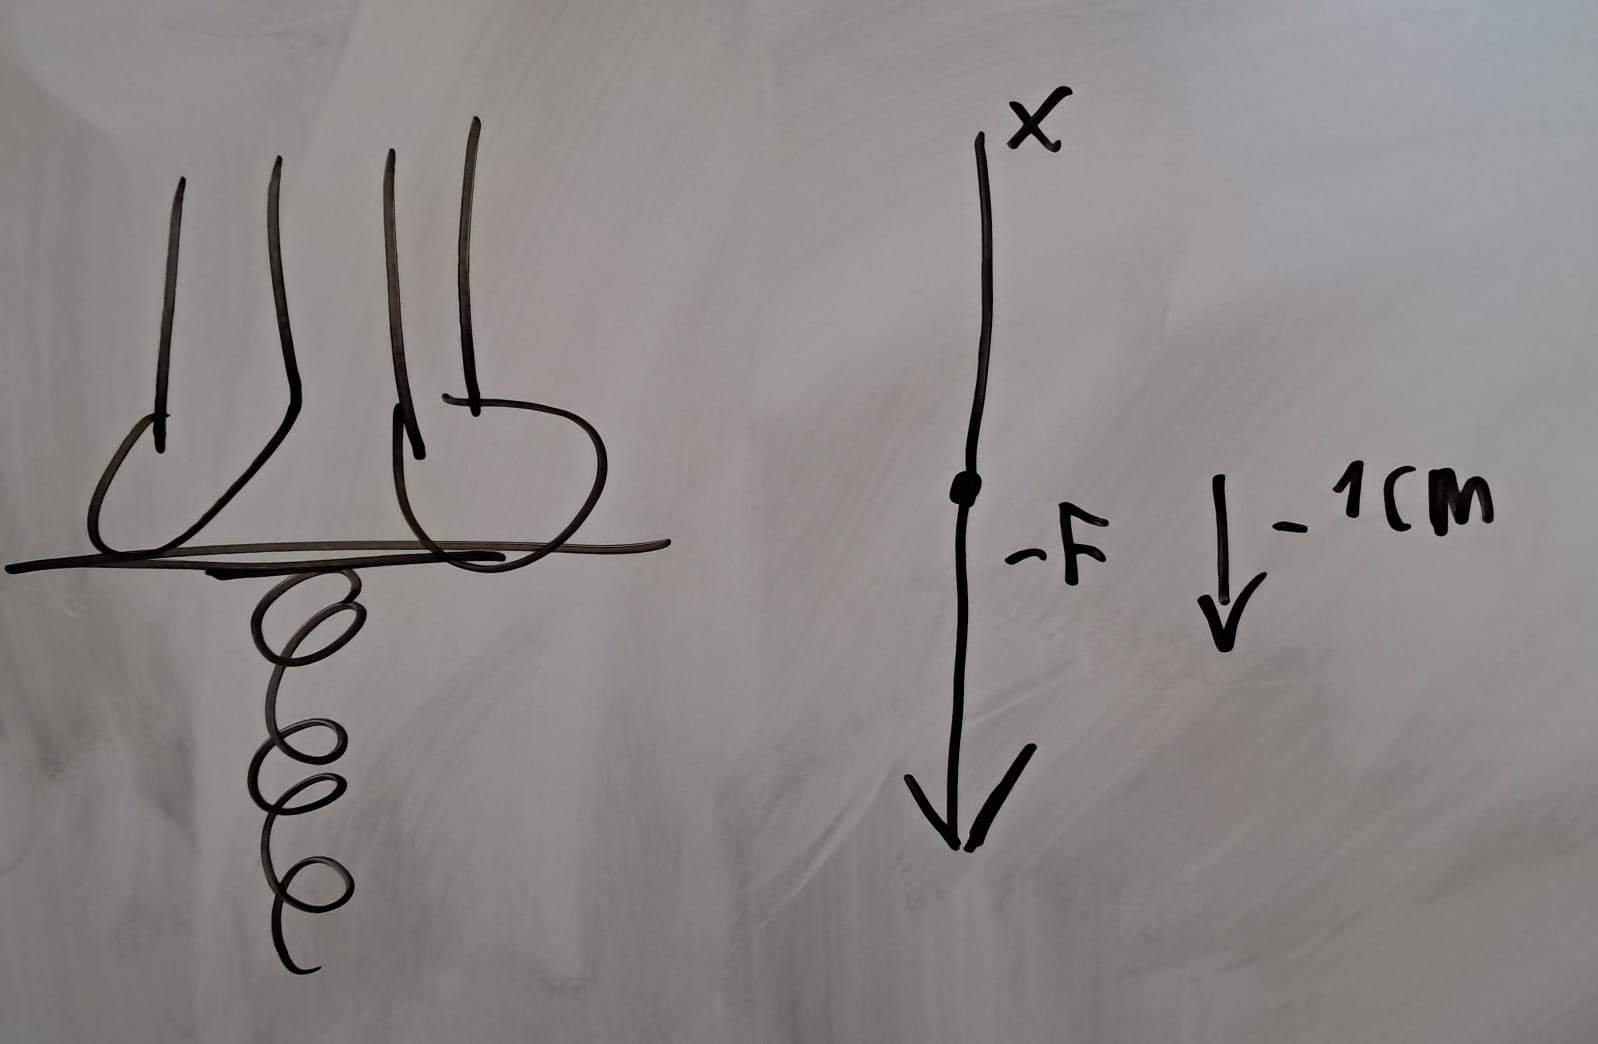
\includegraphics[width=0.6\textwidth]{img/5.3-3.png}
    \end{figure}

    \par Por la ley de Hooke:

    \[ F_x = k x \quad \Longrightarrow \quad k = \frac{F_x}{x} \]

    \par Remplazando tenemos:

    \[ k = \frac{-600 N}{-0.01 m} = 60000 N/m \]

    \par Entonces la constante de fuerza de resorte es de $60000 N/m$.

    \vspace{0.5cm}

    \par Para calcular el trabajo total efectuado sobre el resorte, usaremos la ecuación de trabajo:

    \[ W = \int_{x_1}^{x_2} F_x \, dx = \int_{x_1}^{x_2} k x \, dx = \frac{1}{2} k x_2^2 - \frac{1}{2} k x_1^2 \]

    \par Tomando $x_1 = 0$ y $x_2 = -0.01 m$ tenemos:

    \[ W = \frac{1}{2} \cdot 60000 N/m \cdot (-0.01 m)^2 - \frac{1}{2} \cdot 60000 N/m \cdot 0^2 = 3 J - 0 = 3 J \]

    \[ W = 3 J \]

    \newtitle{Teorema trabajo-energía para movimiento rectilíneo, con fuerzas variables}

    \par En la sección 5.2 dedujimos el teorema trabajo-energía, $W_{tot} = K_2 - K_1$, para el caso específico de movimiento rectilíneo con fuerza neta constante. Ahora podemos demostrar que dicho teorema se cumple aun si la fuerza varía con la posición.
    \par Para ello, recordamos que la aceleración a de una partícula puede expresarse de varias formas. Usando $a_x = {dv_x}/{dt}$, $v_x = dx/dt$ y la regla de la cadena para derivadas:

    \[ a_x = \frac{dv_x}{dt} =  \frac{dv_x}{dx} \frac{dx}{dt} = v_x \frac{dv_x}{dx}  \]

    \par Con este resultado, la ecuación $W_{tot} = \int_{x_1}^{x_2} F_x \, dx$ nos dice que el trabajo total efectuado por la fuerza neta $F_x$ es

    \[ W_{tot} = \int_{x_1}^{x_2} F_x \, dx = \int_{x_1}^{x_2} m a_x \, dx = \int_{x_1}^{x_2} m v_x \frac{dv_x}{dx} \, dx \]

    \par Ahora, ($dv_x/dx$) $dx$ es el cambio de velocidad $dv_x$ durante el desplazamiento $dx$, así
que podemos sustituir $dv_x$ por ($dv_x/dx$) $dx$ en la ecuación. Esto cambia la variable de integración de $x$ a $v_x$, así que cambiamos los límites de $x_1$ y $x_2$ a las velocidades correspondientes $v_1$ y $v_2$ en esos puntos:

    \[ W_{tot} = \int_{v_1}^{v_2} m v_x \, dx \]

    \par La integral de $v_xdv_x$ es $v_x^2/2$. Sustituyendo los límites, tenemos finalmente

    \[ W_{tot} = \frac{1}{2} m v_2^2 - \frac{1}{2} m v_1^2 \]

    \par Ésta es la ecuación que buscabamos. Por lo tanto, el teorema trabajo-energía es válido aun sin el supuesto de que la fuerza neta es constante.

    \definicion{
        \centering
        \( W_{tot} = \int_{v_1}^{v_2} m v_x \, dv_x \quad \quad \text{(Teorema trabajo-energía, con fuerzas variables)} \)
    }

    \newex{Ejercicio 12. Movimiento con fuerza variable}

    \par Un deslizador de riel de aire con masa de $0.100 kg$ se conecta al extremo del riel horizontal con un resorte cuya constante de fuerza es $20.0 N/m$. Inicialmente, el resorte no está estirado y el deslizador se mueve con rapidez de $1.50 m/s$ a la derecha. Calcule la distancia máxima $d$ que el deslizador se mueve a la derecha, 
    
    \begin{list}{}{}
        \item a) si el riel está activado, de modo que no hay fricción; y
        \item b) si se corta el suministro de aire al riel, de modo que hay fricción cinética con coeficiente $\mu_k = 0.47$.
    \end{list}

    \newex{Solución 12.}

    \par Datos:

    \begin{itemize}
        \item $m = 0.100 kg$
        \item $k = 20.0 N/m$
        \item $v_1 = 1.50 m/s$
    \end{itemize}

    \par a) Primero diagramamos el problema:

    \begin{figure}[H]
        \centering
        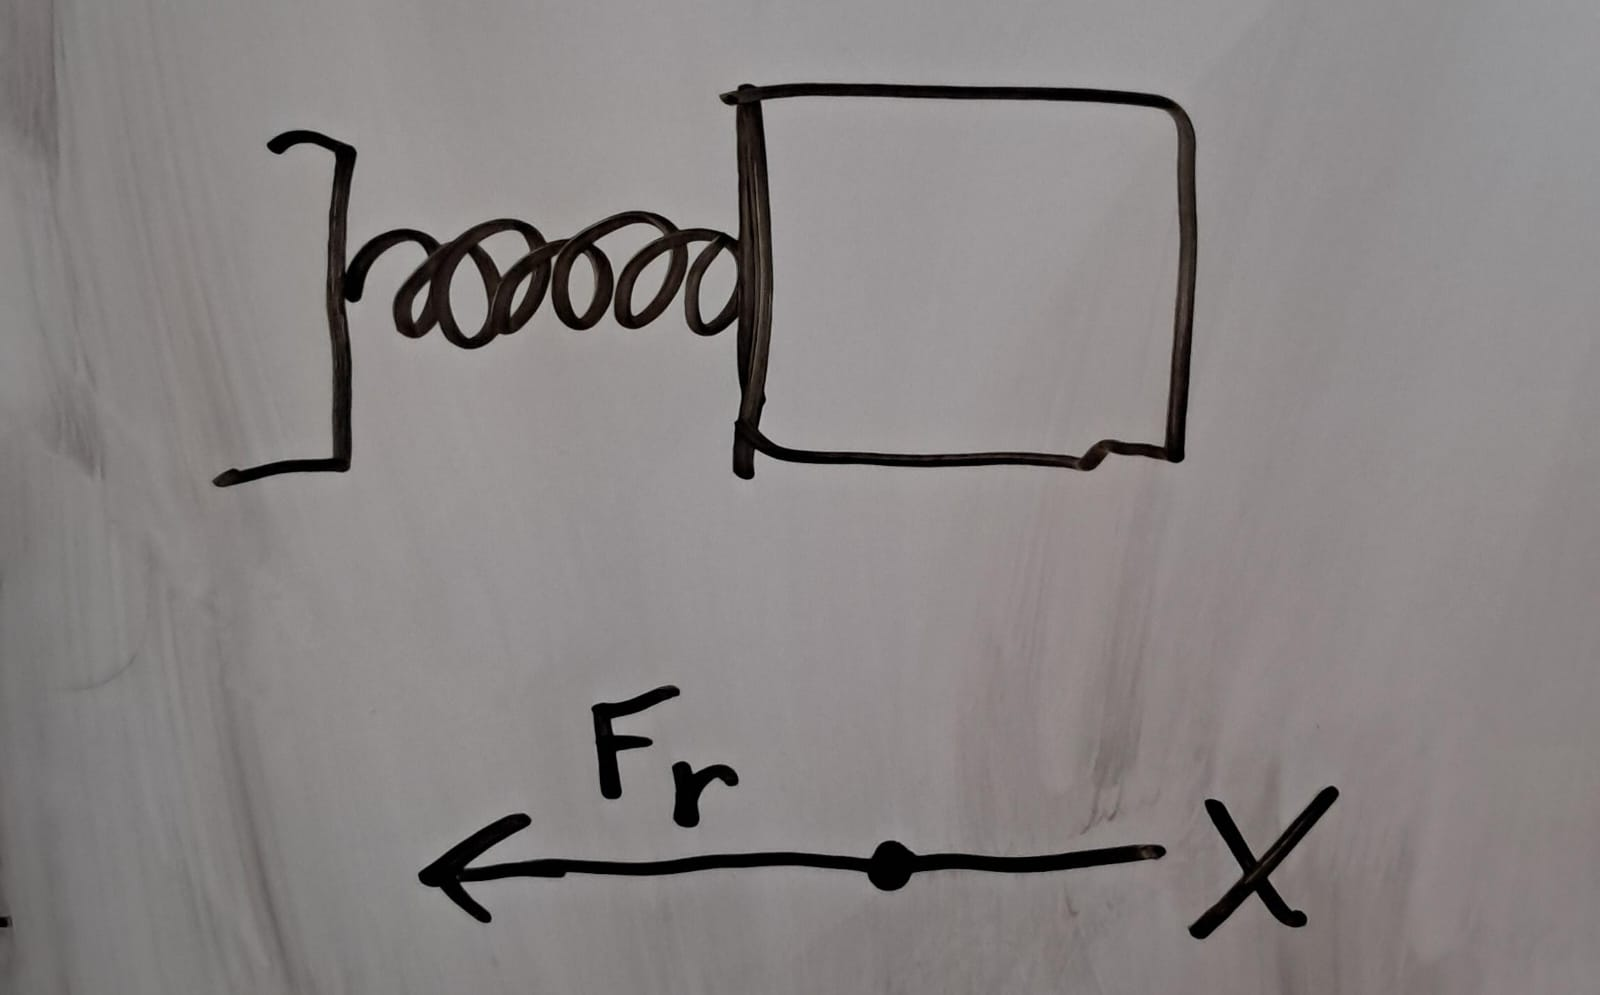
\includegraphics[width=0.5\textwidth]{img/5.3-4.png}
    \end{figure}

    \par el deslizador efectúa sobre el resorte un trabajo dado por la ecuación $ W = \frac{1}{2} k d^2 - \frac{1}{2} k d_0^2 = \frac{1}{2} k d^2 $, y el resorte sobre el deslizador un trabajo igual pero negativo: $-\frac{1}{2} k d^2$ como es el unico trabajo que es ejercido sobre el deslizador entonces $ W_{tot} = -\frac{1}{2} k d^2 $ por lo que utilizando el teorema trabajo-energía, con $K_1 = \frac{1}{2} m v_1^2$ y $K_2 = 0$, ya que la energia cinetica es cero al finalizar el movimiento, tenemos:

    \[ -\frac{1}{2} k d^2 = 0 - \frac{1}{2} m v_1^2 = - \frac{1}{2} m v_1^2 \]

    \[ k d^2 = m v_1^2 \]

    \par Despejamos $d$

    \[ d = \sqrt{\frac{m v_1^2}{k}} = \sqrt{\frac{0.1 kg \cdot (1.5 m/s)^2}{20 N/m}} \approx 0.106 \sqrt{kg \cdot m^2/s^2 \cdot m/N}  \]

    \[ [d] = \sqrt{\cancel{kg} \cdot m^3/\cancel{s^2} \cdot \frac{1}{\cancel{kg} \cdot m/\cancel{s^2}}} = \sqrt{\frac{m^3}{m}} = \sqrt{m^2} = m \]

    \[ d = 0.106 m = 10.6 cm \]

    \par b) Primero diagramamos el problema:

    \begin{figure}[H]
        \centering
        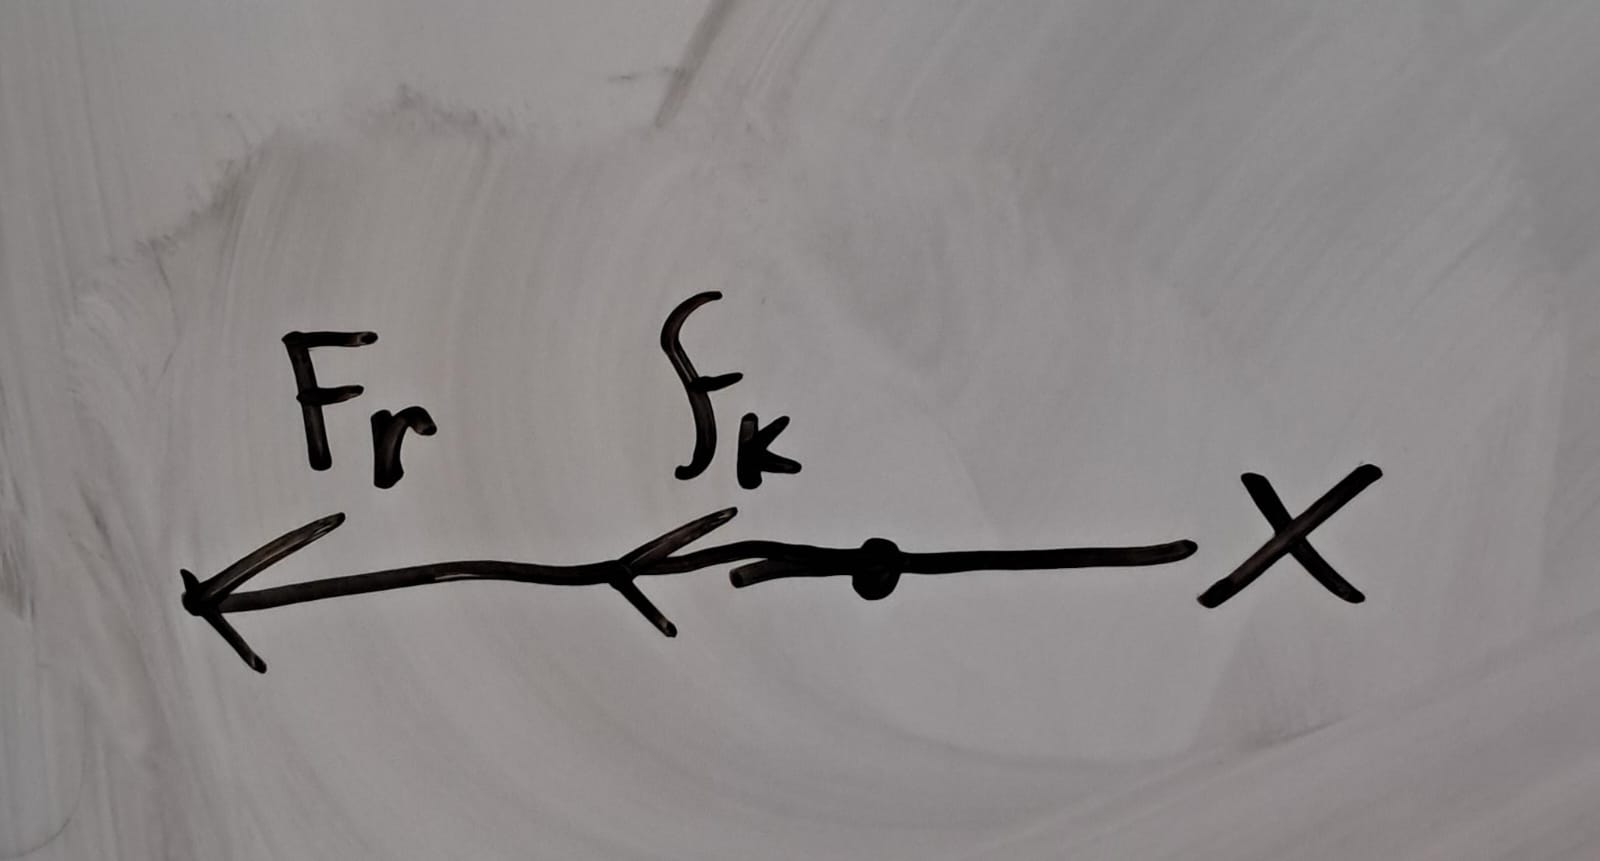
\includegraphics[width=0.5\textwidth]{img/5.3-5.png}
    \end{figure}

    \par Para calcular el trabajo total $W_{tot}$ tenemos que sumar el trabajo que ejerce la fricción cinética sobre el deslizador ($ - f_k d $) y el trabajo que ejerce el resorte sobre el deslizador ($-\frac{1}{2} k d^2$):

    \[ -\frac{1}{2} k d^2 - f_k d = 0 - \frac{1}{2} m v_1^2 \]

    \[ -\frac{1}{2} k d^2 - f_k d + \frac{1}{2} m v_1^2 = 0 \]

    \[ (-10 N/m)d^2 + (-0.46 N)d + (0.11 N \cdot m) = 0 \]

    \par Usamos la ecuación cuadrática para obtener la solución:

    \[ d_{1,2} = \frac{(0.46 N) \pm \sqrt{ (0.46 N)^2 - 4 (-10 N/m) (0.11 N \cdot m)} }{-20 N/m} \]

    \[ d_1 =  0.086 m \quad , \quad d_2 = -0.132 m \]

    \par Como estamos buscando un valor positivo, elegimos $d_1 = 0.086 m = 8.6 cm$

    \newtitle{Teorema trabajo-energía para movimientos en una curva}

    \ladoALado{
        \par Podemos generalizar nuestra definición de trabajo para incluir una fuerza que varía en dirección, no sólo en magnitud, con un desplazamiento curvo. Suponga que una partícula se mueve de P1 a P2 siguiendo una curva, como se muestra en la figura a. Dividimos la curva entre esos puntos en muchos desplazamientos vectoriales infinitesimales, siendo $d\vec{l}$ (diferencial de $\vec{l}$) uno representativo. Sea $\vec{F}$ la fuerza en un punto representativo de la trayectoria, y sea $\phi$ el ángulo entre $\vec{F}$ y $d\vec{l}$ en ese punto. De manera que el elemento pequeño de trabajo $dW$ realizado sobre la partícula durante el desplazamiento $d\vec{l}$ puede escribirse como

        \[ dW = F \cos(\phi) dl = F_{\parallel} dl = \vec{F} \cdot d\vec{l} \]

        \noindent donde $F_{\parallel} = F \cos(\phi)$ es la componente de $\vec{F}$ en la dirección paralela a $d\vec{l}$ (figura b). El trabajo total realizado por F sobre la partícula al moverse de P1 a P2 es, entonces:

    }{img/5.3-6.png}{0.6}{0.4}

    \definicion{
        \centering
        \( W = \int_{P_1}^{P_2} F \cos(\phi) dl = \int_{P_1}^{P_2} F_{\parallel} dl = \int_{P_1}^{P_2} \vec{F} \cdot d\vec{l} \)
    }

    \par ...

    \newex{Ejercicio 13. Movimiento en una trayectoria curva I}

    \par En un día de campo familiar, le piden a usted empujar a su odioso primo Morton en un columpio. El peso de Morton es $w$, la longitud de las cadenas es $R$, y usted lo empuja hasta que las cadenas forman un ángulo $\theta_0$ con la vertical. Para ello, usted ejerce una fuerza horizontal variable $\vec{F}$ que comienza en cero y aumenta gradualmente apenas lo suficiente para que Morton y el columpio se muevan lentamente y permanezcan casi en equilibrio. ¿Qué trabajo total realizan todas las fuerzas sobre Morton? ¿Qué trabajo realiza la tensión $T$ en las cadenas? ¿Qué trabajo efectúa usted aplicando la fuerza $\vec{F}$? (Ignore el peso de las cadenas y el asiento.)

    \newex{Solución 13.}

    \par Diagramamos el problema:

    \begin{figure}[H]
        \centering
        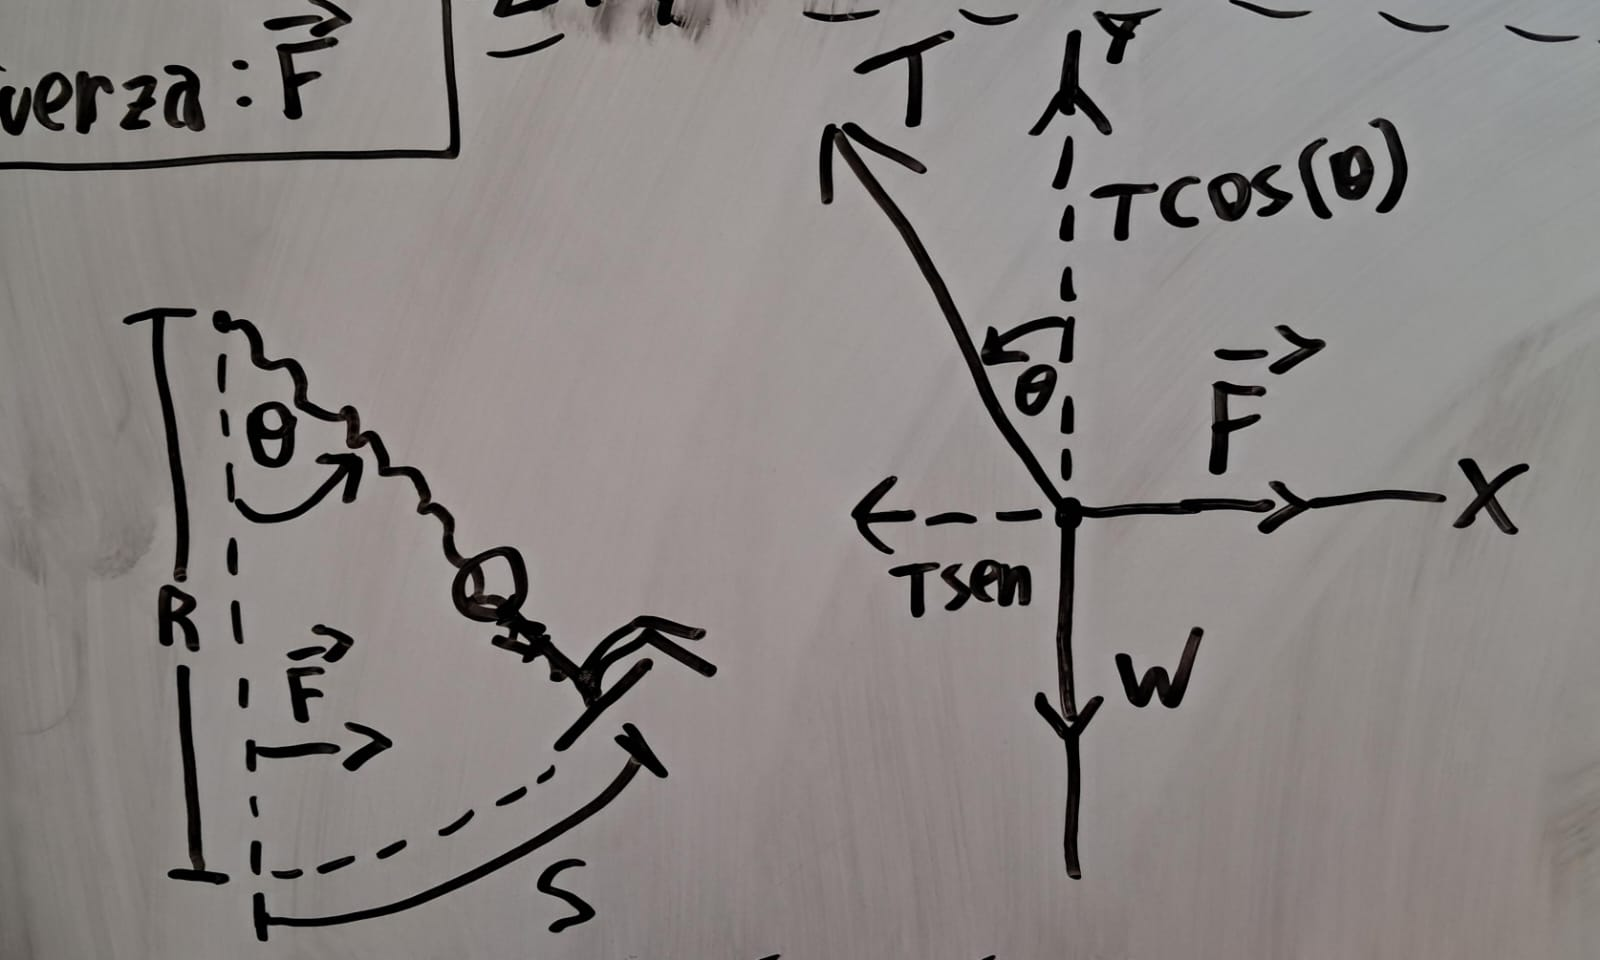
\includegraphics[width=0.5\textwidth]{img/5.3-7.png}
    \end{figure}

    \par Como Morton esta en equilibrio sabemos que $\Sigma F_x = 0$ y $\Sigma F_y = 0$:

    \[ \Sigma F_x = F + (-T \sin(\theta)) = 0 \quad \Longrightarrow \quad F = T \sin(\theta) \]

    \[ \Sigma F_y = T \cos(\theta) + (-w) = 0 \quad \Longrightarrow \quad w = T \cos(\theta) \]

    \par Dividiendo ambas expresiones obtenemos:

    \[ \frac{F}{w} = \frac{\cancel{T} \sin(\theta)}{\cancel{T} \cos(\theta)} = \tan(\theta) \quad \Longrightarrow \quad F = w \tan(\theta) \]

    \par Primero calculamos el trabajo que realiza $\vec{T}$ sobre Morton. Como $\vec{T}$ es perpendicular a la trayectoria $d\vec{l}$, el trabajo realizado es:

    \[ dW = T_{\parallel} dl = T \cos(90^\circ) dl = 0 \cdot dl = 0 \]

    \par Por lo que, el trabajo realizado por la tensión $T$ sobre Morton es 0.

    \vspace{0.5cm}

    \par Ahora calculamos el trabajo realizado por la fuerza $\vec{F}$ sobre Morton. Para ello debemos calcular la longitud del arco $s$ que es igual a $R \theta_0$ ($\theta$ radianes). Por lo tanto el desplazamiento $d\vec{l}$ tiene magnitud $dl = ds = R d\theta$ y el trabajo realizado es:

    \[ W = \int_{P_1}^{P_2} \vec{F} \cdot d\vec{l} = \int_{s_1}^{s_2} F \cos(\theta) ds \]

    \par Remplazando tenemos:

    \[ W = \int_{0}^{\theta_0} (w \tan(\theta)) \cos(\theta) R d\theta = \int_{0}^{\theta_0} w R \sin(\theta) d\theta = w R \int_{0}^{\theta_0} \sin(\theta) d\theta \]

    \par Terminando en

    \[ W = wR (-\cos(\theta_0) + 1)\]

    \par Ahora para calcular el trabajo total realizado por todas las fuerzas sobre Morton tenemos:

    \[ W_{tot} = W_{F} + W_{T} = wR (-\cos(\theta_0) + 1) + 0 = wR (-\cos(\theta_0) + 1) \]

    \newex{Ejercicio 14. Movimiento en una trayectoria curva II}

    \par En el Ejercicio 13, el desplazamiento infinitesimal $d\vec{l}$ tiene magnitud $ds$, su componente $x$ es $ds \cos(\theta)$ y su componente $y$ es $ds \sin(\theta)$. Por lo tanto, $d\vec{l} = \hat{i} [ds \cos(\theta)] + \hat{j} [ds \sin(\theta)]$. Use esta expresión y la ecuación $ W = \int_{P_1}^{P_2} \vec{F} \cdot d\vec{l} $ para calcular el trabajo efectuado durante el movimiento por la tensión de la cadena, por la fuerza de gravedad y por la fuerza F.

    \newex{Solución 14.}

    \par Tenemos $d\vec{l}$ expresados en componentes por lo que nos conviene expresar las fuerzas en componentes:

    \begin{list}{$\bullet$}{}
        \item $ \vec{T} = \hat{i}[-T \sin(\theta)] + \hat{j}[T \cos(\theta)]$
        \item $ \vec{w} = \hat{j}[-w] $
        \item $ \vec{F} = \hat{i}[F] $ 
    \end{list}

    \par Ahora calculamos el producto escalar de las fuerzas con $d\vec{l}$:

    \begin{list}{}{}
        \item $ \vec{T} \cdot d\vec{l} = [-T \sin(\theta)][ds \cos(\theta)] + [T \cos(\theta)][ds \sin(\theta)] = 0 $
        \item $ \vec{w} \cdot d\vec{l} = [-w][ds \sin(\theta)] = -w  \sin(\theta) ds $
        \item $ \vec{F} \cdot d\vec{l} = [F][ds \cos(\theta)] = F \cos(\theta) ds $
    \end{list}

    \par Ahora calculamos el trabajo realizado por el peso:

    \[ W_{w} = \int_{P_1}^{P_2} \vec{w} \cdot d\vec{l} = \int_{P_1}^{P_2} -w \sin(\theta) ds = \int_{0}^{\theta_0} -w \sin(\theta) R d\theta = -w R \int_{0}^{\theta_0} \sin(\theta) d\theta \]

    \[ W_{w} = -w R [ 1 - \cos(\theta_0) ] \]

    \newsubsection{Potencia}

    \par En el habla cotidiana, “potencia” suele emplearse como sinónimo de “energía” o “fuerza”. En física usamos una definición mucho más precisa: potencia es la rapidez con que se efectúa trabajo; al igual que el trabajo y la energía, la potencia es una cantidad escalar.

    \par Si se realiza un trabajo $\Delta W$ en un intervalo $\Delta t$, el trabajo medio efectuado por unidad de tiempo o potencia media $P_{med}$ se define como

    \definicion{
        \centering
        \( P_{med} = \frac{\Delta W}{\Delta t} \) \quad (potencia media)
    }

    \par La rapidez con que se efectúa trabajo quizá no sea constante. Podemos definir la \bl{potencia instantánea} $P$ como el cociente de la ecuación cuando $\Delta t$ se aproxima a cero:

    \definicion{
        \centering
        \( P = \lim_{\Delta t \to 0} \frac{\Delta W}{\Delta t} \) \quad (potencia instantánea)
    }

    \par En el SI la unidad de potencia es el watt ($W$), llamada así por el inventor inglés James Watt. Un watt es igual a un joule por segundo:

    \[ 1 W = 1 J/s \]

    \par En el sistema británico, el trabajo se expresa en pie-libras, y la unidad de potencia es el pie-libra por segundo. También se usa una unidad mayor, el caballo de potencia (hp):

    \[ 1 hp = 550 ft \cdot lb/s \]

    \[ 1 hp = 746 W \]

    \par El watt es una unidad común de potencia \textit{eléctrica}; una bombilla eléctrica de $100 W$ convierte $100 J$ de energía eléctrica en luz y calor cada segundo. Sin embargo, los watts no son inherentemente eléctricos.

    \par En mecánica, también podemos expresar la potencia en términos de fuerza y velocidad.

    \[ P = \frac{F_{\parallel} ds}{dt} = F_{\parallel} \frac{ds}{dt} = F_{\parallel} v \]

    \par donde v es la magnitud de la velocidad instantánea. También podemos expresar la ecuación en términos del producto escalar:

    \definicion{
        \centering
        \( P = \vec{F} \cdot \vec{v} \)
    }

    \newex{Ejercicio 15. Fuerza y potencia}

    \par Cada uno de los dos motores a reacción de un avión Boeing 767 desarrolla un empuje (fuerza hacia adelante sobre el avión) de $197000 N$. Cuando el avión está volando a $250 m/s$ ($900 km/h$), ¿cuántos caballos de potencia desarrolla cada motor?

    \newex{Solución 15.}

    \par...

    \newsection{Energía Potencial y Conservación de la Energía}

    \par Cuando un clavadista se tira de un trampolín a la alberca, golpea el agua rápida­mente, con mucha energía cinética. ¿De dónde proviene esa energía? La res­puesta que dimos en el capítulo 6 fue que la fuerza gravitacional (su peso) realiza trabajo sobre el clavadista al caer. La energía cinética del clavadista —energía asociada con su \textit{movimiento}— aumenta en una cantidad igual al trabajo realizado.

    \par Sin embargo, hay otra forma muy útil de ver el trabajo y la energía cinética. Este nuevo enfoque se basa en el concepto de \textit{energía potencial}, que es energía asociada a la posición de un sistema, no a su movimiento. En este enfoque, hay energía potencial gravitacional incluso cuando el clavadista está parado en el trampolín.

    \par Demostraremos que, en algunos casos, la suma de las energías cinética y potencial de un sistema, llamada, energía mecánica total, es constante durante el movimiento del sistema. Esto nos llevará al enunciado general de la ley de conservación de la energía, que es uno de los principios más fundamentales y trascendentales de la ciencia.

    \newsubsection{Energía potencial gravitacional}

    \par En cualquier interacción, el cambio de energía cinética de una partícula es igual al trabajo total efectuado sobre la partícula por todas las fuerzas que actúan sobre ella.

    \par En muchas situaciones, parece que se almacena energía en un sistema para recuperarse después. Por ejemplo, hay que efectuar trabajo para levantar una roca pesada sobre la cabeza. Parece razonable que, al levantar la roca en el aire, se está almacenando energía en el sistema, la cual se convierte después en energía cinética al dejar caer la roca.

    \vspace{0.5cm}

    \par Este ejemplo señala a la idea de una energía asociada con la posición de los cuerpos en un sistema. Este tipo de energía es una medida del \textit{potencial} o \textit{posibilidad} de efectuar trabajo. Al levantar una roca, existe la posibilidad de que la fuerza de gravitación realice trabajo sobre ella, pero sólo si la roca se deja caer al suelo. Por ello, la energía asociada con la posición se llama \bl{energía potencial}. Lo dicho sugiere que hay energía potencial asociada al peso de un cuerpo y a su altura sobre el suelo: la energía \textit{potencial gravitacional}.

    \par Ahora tenemos \bl{dos} formas de describir lo que sucede cuando un cuerpo cae sin resistencia del aire. Una forma consiste en decir que disminuye la energía potencial gravitacional y aumenta la energía cinética del cuerpo que cae. La otra forma, que vimos en el capítulo 6, es que aumenta la energía cinética de un cuerpo que cae porque la fuerza de gravedad terrestre (el peso del cuerpo) realiza trabajo sobre el cuerpo. Más adelante en esta sección utilizaremos el teorema trabajo-energía para demostrar que estas dos descripciones son equivalentes.

    \ladoALado{
        \par Consideremos un cuerpo de masa m que se mueve en el eje y (vertical), como en la figura.  Las fuerzas que actúan sobre él son su peso, de magnitud $w = mg$, y tal vez otras; llamamos a la suma vectorial (resultante) de todas las otras fuerzas $\vec{F}_{otras}$. Suponemos que el cuerpo permanece tan cerca de la superficie terrestre que el peso es constante. Queremos determinar el trabajo efectuado por el peso cuando el cuerpo cae de una altura $y_1$ sobre el origen a una altura menor $y_2$ (figura a). El peso y el desplazamiento tienen la misma dirección, así que el trabajo $W_{grav}$ efectuado sobre el cuerpo por su peso es positivo;

        \[ W_{grav} = F s = w (y_1 - y_2) = mg y_1 - mg y_2 \]

        \par Esta expresión también da el trabajo correcto cuando el cuerpo sube y $y_2$ es mayor que $y_1$ (figura b). En tal caso, la cantidad $y_1 - y_2$ es negativa y $W_{grav}$ es negativa porque el peso y el desplazamiento tienen direcciones opuestas.

        \par La ecuación muestra que podemos expresar $W_{grav}$ en términos de los valores de la cantidad $mg y$ al principio y al final del desplazamiento. Esta cantidad, el producto del peso $mg$ y la altura $y$ sobre el origen de las coordenadas, es la \bl{energía potencial gravitacional}, $U_{grav}$:

    }{img/6.1-1.png}{0.6}{0.4}

    \definicion{
        \centering
        $U_{grav} = mg y$ \quad \quad \text{(energía potencial gravitacional)}
    }

    \par Su valor inicial es $U_{grav,1} = mg y_1$ y su valor final es $U_{grav,2} = mg y_2$. El cambio en $U_{grav}$ es su valor final menos su valor inicial: $\Delta U_{grav} = U_{grav,2} - U_{grav,1}$. Podemos expresar el trabajo $W_{grav}$ realizado por la fuerza gravitacional durante el desplazamiento de $y_1$ a $y_2$ como

    \definicion{
        \centering
        $ W_{grav} = U_{grav,1} - U_{grav,2} = -( U_{grav,2} - U_{grav,1}) = - \Delta U_{grav} $
    }

    \par El signo negativo de DUgrav es fundamental. Cuando el cuerpo sube, y aumenta, el trabajo realizado por la gravedad es negativo y la energía potencial gravitacional aumenta ($\Delta U{grav} > 0$). Si el cuerpo baja, y disminuye, la gravedad realiza trabajo positivo y la energía potencial gravitacional se reduce ($\Delta U{grav} < 0$).

    \newtitle{Conservación de la energía mecánica (sólo fuerzas gravitacionales)}

    \par Si quiere ver para qué sirve la energía potencial gravitacional, suponga que el peso del cuerpo es la única fuerza que actúa sobre él: $F_{otras} = 0$. Entonces, el cuerpo cae libremente sin resistencia del aire, y podría estar subiendo o bajando. Sea $v_1$ su rapidez en $y_1$ , y $v_2$ en $y_2$. El teorema trabajo-energía indica que el trabajo total efectuado sobre el cuerpo es igual al cambio en su energía cinética; $W_{tot} = \Delta K = K_2 - K_1$. Si la gravedad es la única fuerza que actúa, entonces, $W_{tot} = W_{grav} = -\Delta U_{grav} = U_{grav,1} - U_{grav,2}$. Juntando esto,

    \[ K_2 - K_1 = U_{grav,1} - U_{grav,2} \]

    \noindent que podemos reescribir como

    \definicion{
        \centering
        $ K_1 + U_{grav,1} = K_2 + U_{grav,2} $
    }

    \par Ahora definimos la suma $K + U{grav}$ de las energías cinética y potencial como $E$, la \bl{energía mecánica total del sistema}. Así, $E_1 = K_1 + U_{grav,1}$ es la energía mecánica total en $y_1$ y $E_2 = K_2 + Ugrav,2$ es la energía mecánica total en $y_2$. Entonces podemos decir que $E_1 = E_2$. No obstante, dado que las posiciones $y_1$ y $y_2$ son puntos arbitrarios en el movimiento del cuerpo, la energía mecánica total $E$ tiene el mismo valor en todos los puntos durante el movimiento;

    \[ E = K + U_{grav} = \text{constante} \]

    \par Es decir, \textit{Si sólo la fuerza de gravedad efectúa trabajo, la energía mecánica total es constante, es decir, se conserva}. Éste es nuestro primer ejemplo de la \bl{conservación de la energía mecánica}.

    \begin{figure}[H]
        \centering
        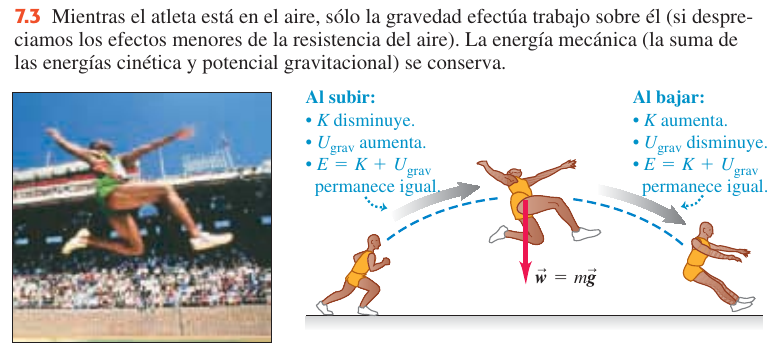
\includegraphics[scale=0.7]{img/6.1-2.png}
    \end{figure}

    \newex{Ejercicio 16. Altura de una pelota por conservación de la energía}

    \par Usted lanza una pelota de béisbol con masa de 0.145 kg hacia arriba, dándole una velocidad inicial hacia arriba de $20.0 m/s$. Determine qué altura alcanza, despreciando la resistencia del aire.

    \newex{Solución 16.}

    \par ...

    \newtitle{Energía potencial gravitacional para movimiento en una trayectoria curva}

    \par Sobre el cuerpo actúa la fuerza gravitacional $\vec{w} = m\vec{g} $ y tal vez otras fuerzas cuya resultante llamamos $\vec{F}_{otras}$. Para calcular el trabajo efectuado por la fuerza gravitacional durante este desplazamiento, dividimos la trayectoria en segmentos pequeños $\Delta \vec{s}$; un segmento típico. El trabajo realizado por la fuerza gravitacional sobre este segmento es el producto escalar de la fuerza y el desplazamiento. En términos de vectores unitarios, la fuerza es $\vec{w} = m\vec{g} = -mg \hat{j}$  y el desplazamento es $\Delta \vec{s} = \Delta x \hat{i} + \Delta y \hat{j}$, así que el trabajo efectuado por la fuerza gravitacional es

    \[ \vec{w} \cdot \Delta \vec{s} = -mg \hat{j} \cdot (\Delta x \hat{i} + \Delta y \hat{j}) = -mg \Delta y \]

    El trabajo efectuado por la gravedad es el mismo que si el cuerpo se hubiera desplazado verticalmente una distancia $\Delta y$, sin desplazamiento horizontal. Esto se cumple para cada segmento, así que el trabajo total efectuado por la fuerza gravitacional es $-mg$ multiplicado por el desplazamiento vertical total ($y_2 - y_1$):

    \[ W_{grav} = -mg(y_2 - y_1) = mg y_1 - mg y_2 = U_{grav,1} - U_{grav,2} \]

    \par Esto es igual a la ecuación (7.1) o (7.3), donde se supuso una trayectoria completamente vertical. Así que, aun si la trayectoria de un cuerpo entre dos puntos es curva, el trabajo total efectuado por la gravedad depende sólo de la diferencia de altura entre esos dos puntos. Por lo tanto, \textit{podemos usar la misma expresión para la energía potencial gravitacional, sea la trayectoria del cuerpo recta o curva}.

    \newex{Ejercicio 17. Cálculo de rapidez en un círculo vertical}

    \par Imagine que su primo Morton baja en patineta por una rampa curva en un parque. Tratando a Morton y a su patineta como una partícula, ésta describe un cuarto de círculo de radio $R = 3.00 m$. La masa total de Morton y su patineta es de $25.0 kg$. Él parte del reposo y no hay fricción. 

    \begin{list}{}{}
        \item a) Calcule su rapidez en la base de la rampa.
        \item b) Obtenga la fuerza normal que actúa sobre él en la base de la rampa.
    \end{list}

    \newex{Solución 17.}

    \par ...

    \newsubsection{Energía potencial elástica}

    \par Describiremos el proceso de almacenar energía en un cuerpo deformable, como un resorte o una banda de hule, en términos de \textit{energía potencial elástica}. Un cuerpo es \textit{elástico} si recupera su forma y tamaño originales después de deformarse.

    \par Procedemos igual que con la energía potencial gravitacional. Comenzamos con el trabajo realizado por la fuerza elástica (del resorte) y lo combinamos con el teorema trabajo-energía. La diferencia es que la energía potencial gravitacional es una propiedad compartida de un cuerpo y la Tierra; no obstante, la energía potencial elástica sólo se almacena en el resorte (u otro cuerpo deformable).

    \ladoALado{

        \par En la figura, el cuerpo está en $x = 0$ con el resorte ni estirado ni comprimido. Movemos el bloque estirando o comprimiendo el resorte, y luego lo soltamos. Al moverse el bloque de una posición $x_1$ a otra posición $x_2$, ¿cuánto trabajo realiza la fuerza elástica (del resorte) sobre el bloque?
        \vspace{0.2cm}
        \par En la sección 5.3 vimos que el trabajo que debemos efectuar sobre el resorte para mover un extremo desde un alargamiento $x_1$ hasta otro alargamiento distinto $x_2$ es
        \[ W = \frac{1}{2} k x_2^2 - \frac{1}{2} k x_1^2 \quad \quad \text{(trabajo efectuado sobre un resorte)}\]
        \vspace{0.2cm}
        \par Ahora nos interesa el trabajo efectuado por el resorte. Por la tercera ley de Newton, un trabajo es el negativo del otro. Cambiando los signos en la ecuación, vemos que, al desplazarse de $x_1$ a $x_2$, el resorte efectúa un trabajo $W_{el}$ dado por
        \[ W_{el} = \frac{1}{2} k x_1^2 - \frac{1}{2} k x_2^2 \quad \quad \text{(trabajo efectuado por el resorte)} \]

    }{img/6.2-1.png}{0.6}{0.4}

    \par Como hicimos con el trabajo gravitacional, podemos expresar el trabajo del resorte en términos de una cantidad dada al principio y al final del desplazamiento. Esta cantidad es $\frac{1}{2} k x^2$, que definimos como la \bl{energía potencial elástica}:

    \definicion{
        \centering
        \( U_{el} = \frac{1}{2} k x^2 \quad \quad \text{(energía potencial elástica)} \)
    }

    \par Podemos usar la ecuación para expresar el trabajo Wel efectuado sobre el bloque por la fuerza elástica en términos del cambio en la energía potencial elástica:

    \definicion{
        \centering
        \( W_{el} = \frac{1}{2} k x_1^2 - \frac{1}{2} k x_2^2 = U_{el,1} - U_{el,2} = - \Delta U_{el} \)
    }

    \par ...

    \newex{Ejercicio 18. Movimiento con fuerzas gravitacional, elástica y de fricción}

    \par ...

    \newsubsection{
        Fuerzas conservativas y no conservativas
    }

    \par Al estudiar la energía potencial se observa que es posible “almacenar” energía cinética convirtiéndola en potencial, con la idea de que luego puede recuperarse en forma de energía cinética. Un ejemplo sencillo es el de una pelota lanzada hacia arriba: en la subida su energía cinética se transforma en potencial, y al descender ocurre el proceso inverso, recuperando la energía cinética. Si no existiera la resistencia del aire, la pelota regresaría al punto de lanzamiento con la misma rapidez con la que fue arrojada.

    \par En el ejemplo se cumple que existe una conversión bidireccional entre energía cinética y energía potencial. Esto permite definir una función de energía potencial de manera que la energía mecánica total, es decir, la suma de la energía cinética y la potencial, es constante o \textit{\bl{se conserva}} durante el movimiento.

    \newtitle{Fuerzas conservativas}

    \par Decimos que una fuerza que ofrece esta oportunidad de conversión bidireccional entre energías cinética y potencial es una \bl{fuerza conservativa}. Hemos visto dos ejemplos de fuerzas conservativas: la gravitacional y la de resorte. Una característica fundamental de las fuerzas conservativas es que su trabajo siempre es \textit{reversible}. Algo que depositamos en el “banco” de energía puede retirarse después sin pérdida.

    \vspace{0.5cm}

    \par El trabajo realizado por una fuerza conservativa siempre tiene estas propiedades:

    \begin{enumerate}
        \item Puede expresarse como la diferencia entre los valores inicial y final de una función de \textit{energía potencial}.
        \item Es reversible.
        \item Es independiente de la trayectoria del cuerpo y depende sólo de los puntos inicial y final.
        \item Si los puntos inicial y final son el mismo, el trabajo total es cero.
    \end{enumerate}

    \par Si las únicas fuerzas que efectúan trabajo son conservativas, la energía mecánica total $E = K + U$ es constante.

    \newtitle{Fuerzas no conservativas}

    \par El trabajo realizado por una \bl{fuerza no conservativa} no puede representarse con una función de energía potencial. Algunas fuerzas no conservativas, como la fricción cinética o la resistencia de fluidos, hacen que se pierda o se disipe energía mecánica: son \bl{fuerzas disipadoras}. 
    
    \par También hay fuerzas no conservativas que \textit{aumentan} la energía mecánica. Los fragmentos de un petardo que estalla salen despedidos con una energía cinética muy grande, debido a una reacción química de la pólvora con el oxígeno. Las fuerzas liberadas por esta reacción no son conservativas porque el proceso no es reversible.

    \newex{Ejercicio 19. El trabajo de fricción depende de la trayectoria}

    \par ...

    \newtitle{La ley de conservación de la energía}

    \par Las fuerzas no conservativas no pueden representarse en términos de energía potencial; no obstante, podemos describir sus efectos en términos de energías distintas de la cinética y la potencial. Cuando un automóvil con frenos bloqueados se derrapa hasta detenerse, se calientan los neumáticos y el camino. La energía asociada a este cambio en el estado de los materiales se denomina \bl{energía interna}. Cuando se eleva la temperatura de un cuerpo, aumenta su energía interna; si se reduce su temperatura, disminuye su energía interna.

    \par Para captar el significado de la energía interna, consideremos un bloque que se desliza por una superficie áspera. Cuando se desliza, la fricción realiza trabajo negativo sobre el bloque, y el cambio de energía interna del bloque y la superficie es positivo (ambos se calientan). Experimentos cuidadosos demuestran que el aumento en la energía interna es exactamente igual al valor absoluto del trabajo efectuado por la fricción. Dicho de otro modo,

    \[ \Delta U_{int} = - W_{otras} \]

    \noindent donde $\Delta U_{int}$ es el cambio de energía interna. Si sustituimos esto en la ecuación $ K_1 + U_1 + W_{otras} = K_2 + U_2 $, vemos que

    \[ K_1 + U_1 - \Delta U_{int} = K_2 + U_2 \]

    \noindent Si escribimos $ \Delta K = K_2 - K_1 $ y $ \Delta U = U_2 - U_1 $, podemos expresar finalmente esto como

    \definicion{
        \centering
        \( \Delta K + \Delta U + \Delta U_{int} = 0 \quad \quad \text{(ley de conservación de la energía)} \)
    }

    \par Este notable enunciado es la forma general de la \bl{ley de conservación de la energía}. En un proceso dado, las energías cinética, potencial e interna de un sistema pueden cambiar; pero la suma de todos los cambios siempre es cero. 
    \par Una disminución en una forma de energía se compensa con un aumento en las otras. Si ampliamos nuestra definición de energía para incluir la energía interna, la ecuación dice que \textit{\bl{la energía nunca se crea ni se destruye, sólo cambia de forma}}. No se ha observado aún una excepción a esta regla.

    \newex{Ejercicio 20. Trabajo efectuado por la fricción}

    \par ...

    \newsubsection{Fuerza y energía potencial}

    \par En los dos tipos de fuerzas conservativas (gravitacional y elástica) que estudiamos, comenzamos con una descripción del comportamiento de la fuerza y de él dedujimos una expresión para la \textit{energía potencial}.
    \par No obstante, en su estudio de la física el lector encontrará situaciones donde tiene una expresión para la \textit{energía potencial} en función de la posición y necesita determinar la \textit{fuerza} correspondiente. Veremos varios ejemplos de este tipo cuando estudiemos las fuerzas eléctricas más adelante. En general, es mucho más fácil calcular primero la energía potencial eléctrica, y luego determinar la fuerza eléctrica correspondiente.

    \vspace{0.5cm}

    \par Veamos cómo calcular la fuerza que corresponde a una expresión de energía potencial dada. Primero, consideremos un movimiento rectilíneo sobre el eje $x$. Denotamos la componente x de la fuerza, que es función de $x$, con $F_x(x)$; y la energía potencial, con $U(x)$. Esta notación nos recuerda que tanto $F_x$ como $U$ son funciones de $x$. Ahora recordamos que, en cualquier desplazamiento, el trabajo $W$ efectuado por una fuerza conservativa es el negativo del cambio de energía potencial $\Delta U$:

    \[ W = - \Delta U \]

    \par Apliquemos esto a un desplazamiento pequeño $\Delta x$. El trabajo efectuado por $F_x(x)$ durante este desplazamiento es aproximadamente igual a $F_x(x) \Delta x$. Decimos “aproximadamente” porque $F_x(x)$ podría variar un poco en el intervalo Dx; pero se cumple, al menos aproximadamente, que

    \[ F_x(x) \Delta x = - \Delta U \quad\quad \text{y} \quad\quad F_x(x) = - \frac{\Delta U}{\Delta x} \]

    \par En el límite $\Delta x \rightarrow 0$, la variación de $F_ x$ se hace despreciable y tenemos la relación exacta

    \definicion{
        \centering
        \( F_x(x) = - \frac{d U(x)}{dx} \quad o \quad F_x(x) = - U'(x) \quad \quad \text{(fuerza a partir de la energía potencial)} \)
    }

    \par El significado físico de la ecuación es que \textit{una fuerza conservativa siempre trata de llevar el sistema a una energía potencial menor}.

    \par Como verificación, consideremos la función de la energía potencial elástica, $U(x) = \frac{1}{2} kx^2$. Si sustituimos por esto:

    \[ F_x(x) = - \frac{d}{dx} \left( \frac{1}{2} kx^2 \right)  = - kx \]

    \newex{Ejercicio 21. Fuerza eléctrica y su energía potencial}

    \par ...

    \newtitle{Fuerza y energía potencial en tres dimensiones}

    \par Podemos extender este análisis a tres dimensiones, donde la partícula puede moverse en las direcciones $x$, $y$, $z$, o todas a la vez. Donde bajo el mismo procedimiento llegamos a:

    \[ F_x(x) = - \frac{\Delta U}{\Delta x} \quad F_y(y) = - \frac{\Delta U}{\Delta y} \quad F_z(z) = - \frac{\Delta U}{\Delta z} \]

    \par Si queremos que las relaciones sean exactas, deberemos tomar límites $\Delta x \rightarrow 0$, $\Delta y \rightarrow 0$ y $\Delta z \rightarrow 0$ para que estos cocientes se conviertan en derivadas.  Calculamos la derivada de $U$ con respecto a $x$ suponiendo que $y$ y $z$ son constantes y sólo $x$ varía, y así sucesivamente. Éstas se llaman derivadas parciales y su notación usual es $\frac{\partial U}{\partial x}$ y así sucesivamente; el símbolo $\partial$ es una d modificada, por lo que escribimos

    \definicion{
        \centering
        \( F_x = - \frac{\partial U}{\partial x} \quad F_y = - \frac{\partial U}{\partial y} \quad F_z = - \frac{\partial U}{\partial z} \)
    }

    \par Podemos usar vectores unitarios para escribir una sola expresión vectorial compacta para la fuerza $\vec{F}$:

    \definicion{
        \centering
        \( \vec{F} = - \left( \frac{\partial U}{\partial x} \hat{i} + \frac{\partial U}{\partial y} \hat{j} + \frac{\partial U}{\partial z} \hat{k} \right) \quad \quad \text{(fuerza a partir de la energía potencial)} \)
    }

    \par La expresión en paréntesis representa una operación específica sobre la función U, donde se obtiene la derivada parcial de U con respecto a cada coordenada, se multiplican por el vector unitario correspondiente y se suman vectorialmente. Esta operación se denomina gradiente de U y  suele abreviarse $\vec{\nabla} U$. Por lo tanto, la fuerza es el negativo del gradiente de la función de energía potencial:

    \[ \vec{F} = - \vec{\nabla} U\]

    \newex{ Ejercicio 22. Fuerza y energía potencial en dos dimensiones}

    \par ...

    \newsubsection{Diagramas de energía}

    \par ...

    \newsection{Momento lineal, impulso y choques}

    \par Hay muchas preguntas relacionadas con fuerzas que no pueden contestarse aplicando directamente la segunda ley de Newton, $\Sigma \vec{F} = m \vec{a}$. Por ejemplo, si un camión de 18 ruedas choca de frente con un auto compacto, ¿qué determina hacia dónde se mueven los restos después del choque? Cuando usted juega billar, ¿cómo decide la dirección que debe dar a la bola blanca para meter la bola 8 en una buchaca?

    \par Algo que tienen en común todas estas preguntas es que implican fuerzas acerca de las que sabemos muy poco: las fuerzas que actúan entre el auto y el camión o entre las dos bolas de billar. Lo curioso es que en este capítulo veremos que ¡no necesitamos saber \textit{nada} acerca de esas fuerzas para contestar preguntas de este tipo!

    \vspace{0.3cm}

    \par Nuestro enfoque utiliza dos conceptos nuevos, \textit{\bl{momento lineal}} e \textit{\bl{impulso}}, y una nueva ley de conservación, la de \textit{\bl{conservación del momento lineal}}, tan importante como la de conservación de la energía. 
    
    \par En el ámbito de la mecánica newtoniana, la conservación del momento lineal nos permite analizar muchas situaciones que serían muy difíciles si tratáramos de aplicar las leyes de Newton directamente. Entre ellas están los choques, en los que dos cuerpos ejercen, uno sobre el otro, fuerzas muy grandes durante un lapso muy breve.

    \newsubsection{Momento lineal e impulso}

    \par En el capítulo 6 reexpresamos la segunda ley de Newton para una partícula, $\Sigma \vec{F} = m \vec{a}$, en términos del teorema del trabajo y la energía, el cual nos ayudó a resolver muchos problemas y nos llevó a la ley de conservación de la energía. Volvamos a $\Sigma \vec{F} = m \vec{a}$ y veamos otra forma útil de replantear esta ley fundamental.

    \newtitle{Segunda ley de Newton en términos del momento lineal}

    \par Consideremos una partícula de masa constante m. Puesto que $\vec{a} = \frac{d \vec{v}}{dt}$, podemos escribir la segunda ley de Newton para esta partícula así:

    \[ \Sigma \vec{F} = m \frac{d \vec{v}}{dt} = \frac{d}{dt} \left( m \vec{v} \right) \]

    \par Así, la segunda ley de Newton dice que la fuerza neta $\Sigma F$ que actúa sobre una partícula es igual a la rapidez de cambio de la combinación $m \vec{v}$, el producto de la masa y la velocidad de la partícula. Llamamos a esta combinación \bl{momento lineal} de la partícula

    \definicion{
        \centering
        \( \vec{p} = m \vec{v} \quad \quad \text{(definición de momento lineal)} \)
    }

    \par Si sustituimos  la definición de momento lineal, en la segunda ley de Newton, tenemos:

    \definicion{
        \centering
        \( \Sigma \vec{F} = \frac{d \vec{p}}{dt} \quad \quad \text{(segunda ley de Newton en términos de momento lineal)} \)
    }

    \par Ésta, y no $\Sigma \vec{F} = m \vec{a}$, es la forma en que Newton planteó originalmente su segunda ley (aunque él llamó momentum al momento lineal), y sólo es válida en marcos de referencia inerciales.

    \newtitle{Teorema del impulso y el momento lineal}

    \par El momento lineal de una partícula $\vec{p} = m \vec{v}$ y su energía cinética $K = \frac{1}{2}mv^2$ dependen de la masa y la velocidad de la partícula. ¿Qué diferencia fundamental hay entre estas cantidades? Para ver la diferencia física entre momento lineal y energía cinética, necesitamos definir una cantidad íntimamente relacionada con el momento lineal: el \textit{impulso}.

    \par Consideremos primero una partícula sobre la que actúa una fuerza neta constante $\Sigma F$ durante un tiempo $\Delta t$, de $t_1$ a $t_2$. El \bl{impulso} de la fuerza neta, denotado con $\vec{J}$, se define como el producto de la fuerza neta y el intervalo de tiempo:

    \definicion{
        \centering
        \( \vec{J} = \Sigma F (t_2 - t_1) = \Sigma F \Delta t \)
    }

    \par Para ver para qué nos sirve el impulso, volvamos a la segunda ley de Newton planteada en términos de momento lineal. Si la fuerza neta $\Sigma F$ es constante, $\frac{d \vec{p}}{dt}$ también es constante. En tal caso, $\frac{d \vec{p}}{dt}$ es igual al cambio total de momento lineal $\vec{p}_2 - \vec{p}_1$ durante el lapso $t_2 - t_1$, dividido entre el lapso:

    \[ \Sigma \vec{F} = \frac{\vec{p}_2 - \vec{p}_1}{t_2 - t_1} \]

    \par Si multiplicamos esta ecuación por ($t_2 - t_1$), tenemos

    \[ \Sigma \vec{F} (t_2 - t_1) = \vec{p}_2 - \vec{p}_1 \]

    \par Obteniendo un resultado conocido como \bl{teorema del impulso y el momento lineal}:

    \definicion{
        \centering
        \( \vec{J} = \vec{p}_2 - \vec{p}_1 \quad \quad \text{(teorema del impulso y el momento lineal)} \)
    }

    \definicion{
        \bl{El cambio del momento lineal de una partícula durante un intervalo de tiempo es igual al impulso de la fuerza neta que actúa sobre la partícula durante ese intervalo.}
    }

    \par El teorema del impulso y el momento lineal también se cumple si las fuerzas no son constantes. Para comprobarlo, integramos los dos miembros de la segunda ley de Newton $\Sigma \vec{F} = \frac{d \vec{p}}{dt}$ con respecto al tiempo entre los límites $t_1$ y $t_2$:

    \[ \int_{t_1}^{t_2} \Sigma \vec{F} dt = \int_{t_1}^{t_2} \frac{d \vec{p}}{dt} dt = \int_{\vec{P}_1}^{\vec{P}_2} d \vec{p} = \vec{p}_2 - \vec{p}_1 \]

    \par La integral de la izquierda es, por definición, el impulso $\vec{J}$ de la fuerza neta $\Sigma \vec{F}$ durante este intervalo:

    \definicion{
        \centering
        \( \vec{J} = \int_{t_1}^{t_2} \Sigma \vec{F} dt \quad \quad \text{(definición general de impulso)} \)
    }

    \newtitle{Comparación de momento lineal y energía cinética}

    \par El teorema del impulso y el momento lineal $\vec{J} = \vec{p}_2 - \vec{p}_1$ dice que los cambios en el momento lineal de una partícula se deben al impulso, que depende del tiempo durante el que actúa la fuerza neta. En cambio, el teorema del trabajo y la energía $W_{tot} = K_2 - K_1$ nos dice que la energía cinética cambia cuando se realiza trabajo sobre una partícula; el trabajo total depende de la distancia en la que actúa la fuerza neta. 

    \par Considere una partícula que parte del reposo en $t_1$, de manera que $\vec{v}_1 = 0$. Su momento lineal inicial es $\vec{p}_1 = m \vec{v}_1 = 0$, y su energía cinética inicial es $K_1 = \frac{1}{2} m v_1^2 = 0$. Ahora, una fuerza neta constante igual a $\vec{F}$ actúa sobre el cuerpo del tiempo $t_1$ al tiempo $t_2$. En este intervalo, la partícula se mueve una distancia $s$ en la dirección de la fuerza. Por lo que el momento lineal del cuerpo en el instante $t_2$ es

    \[ \vec{p}_2 = \vec{p}_1 + \vec{J} = \vec{J} \]

    \noindent donde $\vec{J} = \vec{F} (t_2 - t_1)$ es el impulso que actúa sobre la partícula. Así, el momento lineal de una partícula es igual al impulso que la aceleró desde el reposo hasta su rapidez actual; el impulso es el producto de la fuerza neta que aceleró el cuerpo y el tiempo requerido para la aceleración. En cambio, la energía cinética del cuerpo en $t_2$ es $K_2 = W_{tot} = F s$, el trabajo total efectuado sobre el cuerpo para acelerarlo desde el reposo. El trabajo total es igual al producto de la fuerza neta y la distancia necesaria para acelerar la partícula.

    \newex{Ejercicio 23. Momento lineal contra energía cinética}

    \par Suponga que lanza una pelota de $0.40 kg$ contra una pared, a la cual golpea moviéndose horizontalmente hacia la izquierda a $30 m/s$ y rebotando horizontalmente a la derecha con rapidez de $20 m/s$.

    \begin{list}{}{}
        \item a) Calcule el impulso de la fuerza neta sobre la pelota durante el choque.
        \item b) Si la pelota está en contacto con la pared durante $0.010 s$, calcule la fuerza horizontal media que la pared ejerce sobre la pelota durante el impacto.
    \end{list}

    \newex{Solución 23.}

    \par ...

    \newsubsection{Conservación del momento lineal}

    \par El concepto de momento lineal tiene especial importancia en situaciones en las que dos o más cuerpos \textit{interactúan}. Para ver por qué, consideremos primero un sistema idealizado de dos cuerpos que interactúan entre sí, por ejemplo, dos astronautas que se tocan mientras flotan libremente en el espacio exterior en un ambiente de gravedad cero. Consideremos a los astronautas como partículas. Cada partícula ejerce una fuerza sobre la otra. Los \textit{impulsos} que actúan sobre las dos partículas son iguales y opuestos, y los cambios de momento lineal de las dos partículas serán iguales y opuestos.

    \par Repasemos esto a la luz de ciertos términos nuevos. En cualquier sistema, las fuerzas que las partículas del sistema ejercen entre sí se denominan \bl{fuerzas internas}; las ejercidas sobre cualquier parte del sistema por algún objeto externo son \bl{fuerzas externas}. Las fuerzas internas son $\vec{F}_{B \rightarrow A}$, ejercida por la partícula $B$ sobre la $A$, y $\vec{F}_{A \rightarrow B}$ ejercida por la partícula $A$ sobre la $B$. No hay fuerzas externas, así que tenemos un \bl{sistema aislado}.
    \par Las razones de cambio del momento lineal de ambas partículas son

    \[ \vec{F}_{B \rightarrow A} = \frac{d \vec{p}_A}{dt} \quad\quad \vec{F}_{A \rightarrow B} = \frac{d \vec{p}_B}{dt} \]

    \noindent  las dos fuerzas, $\vec{F}_{B \rightarrow A}$ y $\vec{F}_{A \rightarrow B}$ siempre son iguales en magnitud y opuestas en dirección. Es decir, $\vec{F}_{B \rightarrow A} = - \vec{F}_{A \rightarrow B} $, así que $\vec{F}_{B \rightarrow A} + \vec{F}_{A \rightarrow B} = 0$. Sumando las dos ecuaciones, tenemos

    \[ \vec{F}_{B \rightarrow A} + \vec{F}_{A \rightarrow B} = \frac{d \vec{p}_A}{dt} + \frac{d \vec{p}_B}{dt} = \frac{d (\vec{p}_A + \vec{p}_B)}{dt} = 0 \]

    \par Las razones de cambio de los dos momentos lineales son iguales y opuestas, así que la razón de cambio de la suma vectorial $\vec{p}_A + \vec{p}_B$ es cero. Ahora definimos el \bl{momento lineal total} $\vec{P}$ del sistema de dos partículas como la suma vectorial de los momentos lineales de las partículas individuales. Esto es,

    \[ \vec{P} = \vec{p}_A + \vec{p}_B \]

    \par Así, la ecuación se convierte finalmente en

    \[ \vec{F}_{B \rightarrow A} + \vec{F}_{A \rightarrow B} = \frac{d \vec{P}}{dt} = 0 \]

    \par La razón de cambio del momento lineal total $\vec{P}$ es cero. Por lo tanto, el momento lineal total del sistema es constante, aunque los momentos lineales individuales de las partículas que constituyen el sistema pueden cambiar.

    \definicion{
        \par \bl{Si la suma vectorial de las fuerzas externas sobre un sistema es cero, el momento lineal total del sistema es constante.}
    }

    \par Ésta es la forma más sencilla del \bl{principio de conservación del momento lineal}, el cual es una consecuencia directa de la tercera ley de Newton.
    \par Podemos generalizar este principio para un sistema con cualquier número de partículas $A$, $B$, $C$, … que sólo interactúan entre sí. El momento lineal total del sistema es

    \[ \vec{P} = \vec{p}_A + \vec{p}_B + \vec{p}_C + \cdots = m_A \vec{v}_A + m_B \vec{v}_B + m_C \vec{v}_C + \cdots \quad \text{(momento lineal total del sistema)} \]

    \newex{Ejercicio 24. Retroceso de un rifle}

    \par Un tirador sostiene holgadamente un rifle de masa $m_R = 3.00 kg$, de manera que pueda retroceder libremente al hacer un disparo. Dispara una bala de masa $m_B = 5 g = 0.005 kg$ con una velocidad horizontal relativa al suelo de $v_{Bx} = 300 m/s$. ¿Qué velocidad de retroceso $v_{Rx}$ tiene el rifle? ¿Qué momento lineal y energía cinética finales tiene la bala? ¿Y el rifle?

    \newex{Solución 24.}

    \par ...

    \newsubsection{Conservación del momento lineal y choques}

    \par El término choque hace que una persona común piense en un percance de tráfico. Usaremos el término en ese sentido, pero además ampliaremos su significado para incluir cualquier interacción vigorosa entre cuerpos con duración relativamente corta.

    \par Si las fuerzas entre los cuerpos son mucho mayores que las externas, como suele suceder en los choques, podemos ignorar las fuerzas externas y tratar los cuerpos como un sistema \textit{aislado}. Entonces, el momento lineal se conserva y el momento lineal total del sistema tendrá el mismo valor antes y después del choque.

    \newtitle{Choques elásticos e inelásticos}

    \par Si las fuerzas entre los cuerpos son \textit{conservativas}, de manera que no se pierde ni gana energía mecánica en el choque, la \textit{energía} cinética total del sistema es la misma antes y después. Esto se denomina \bl{choque elástico}. Un choque entre dos canicas o dos bolas de billar es casi totalmente elástico.

    \par Un choque en el que la energía cinética total final es \textit{menor} que la inicial es un \bl{choque inelástico}. Una albóndiga que cae en un plato de espagueti y una bala que se incrusta en un bloque de madera son ejemplos de choques inelásticos. Un choque inelástico en el que los cuerpos se pegan y se mueven como uno solo después del choque es un \bl{choque totalmente inelástico}.

    \vspace{1cm}

    \par \bl{En todo choque en el que se pueden ignorar las fuerzas externas, el momento lineal se conserva y el momento lineal total es el mismo antes y después. La energía cinética total sólo es igual antes y después si el choque es elástico.}

    \newtitle{Choque totalmente inelásticos}

    \ladoALado{
        \par Veamos qué sucede con el momento lineal y la energía cinética en un choque totalmente inelástico de dos cuerpos $A$ y $B$, como en la figura. Dado que los cuerpos quedan pegados después del choque, tienen la misma velocidad final $\vec{v}_2$:

        \[ \vec{v}_A2 = \vec{v}_B2 = \vec{v}_2 \]

        \par La conservación del momento lineal da la relación

        \[ m_A \vec{v}_{A1} + m_B \vec{v}_{B1} = (m_A + m_B) \vec{v}_2 \]

        \par Si conocemos las masas y las velocidades iniciales, podremos calcular la velocidad final común $\vec{v}_2$.

    }{img/7.3-1.png}{0.5}{0.5}

    \newex{Ejercicio 25. Choque totalmente inelástico}

    \par Suponga que, en el choque descrito en el ejemplo 8.5 (sección 8.2), los deslizadores no rebotan, sino que quedan pegados después del choque. Las masas y velocidades iniciales son las mismas que en el ejemplo 8.5. Calcule la velocidad final común v2x y compare las energías cinéticas inicial y final del sistema.

    \newex{Solución 25.}

    \par ...

    \newtitle{Clasificación de los choques}

    \par Es importante recordar que los choques se clasifican de acuerdo con consideraciones de energía. Un choque en el que la energía cinética se \textit{conserva} se considera \textit{\bl{elástico}}. Un choque en el que la energía cinética total \textit{disminuye} se llama \textit{\bl{inelástico}}. Cuando dos cuerpos tienen una \textit{velocidad final común}, decimos que el choque es \textit{\bl{totalmente inelástico}}. También hay casos en los que la energía cinética final es mayor que el valor inicial, por ejemplo el retroceso de los rifles.

    \newsubsection{Choques elásticos}

    \par Como vimos en la sección 7.3, un choque elástico en un sistema aislado es uno en el que se conserva la energía cinética. Estos choques ocurren cuando las fuerzas entre los cuerpos que chocan son conservativas. Si chocan dos bolas de billar, se aplastan un poco cerca del punto de contacto, pero luego rebotan. Parte de la energía cinética se almacena temporalmente como energía potencial elástica, pero al final se convierte una vez más en energía cinética.

    \par Examinemos un choque elástico entre dos cuerpos A y B. Comencemos con un choque en una dimensión, con todas las velocidades en la misma línea, a la que llamamos eje $x$. Llamamos $v_{A1x}$ y $v_{B1x}$ a las componentes $x$ de velocidad antes del choque, y $v_{A2x}$ y $v_{B2x}$ a las componentes $x$ después del choque. Por la conservación de la energía cinética tenemos

    \[ \frac{1}{2} m_A v_{A1x}^2 + \frac{1}{2} m_B v_{B1x}^2 = \frac{1}{2} m_A v_{A2x}^2 + \frac{1}{2} m_B v_{B2x}^2 \]

    \par y la conservación del momento lineal da

    \[ m_A v_{A1x} + m_B v_{B1x} = m_A v_{A2x} + m_B v_{B2x} \]

    \par Si conocemos las masas $m_A$ y $m_B$ y las velocidades iniciales $v_{A1x}$ y $v_{B1x}$, podremos resolver las ecuaciones para obtener las velocidades finales $v_{A2x}$ y $v_{B2x}$.

    \newtitle{Choques elásticos, un cuerpo inicialmente en reposo}

    \par La solución general de las ecuaciones anteriores es algo complicada, así que nos concentraremos en el caso especial en que el cuerpo $B$ está en reposo antes del choque. Piense que el cuerpo B es el blanco que A debe golpear. Las ecuaciones de conservación de energía cinética y el momento lineal son, respectivamente,

    \[ \frac{1}{2} m_A v_{A1x}^2 = \frac{1}{2} m_A v_{A2x}^2 + \frac{1}{2} m_B v_{B2x}^2 \]

    \[ m_A v_{A1x} = m_A v_{A2x} + m_B v_{B2x} \]

    \par Reacomodemos primero las ecuaciones así:

    \[ m_B v_{B2x}^2 = m_A (v_{A1x} - v_{A2x})(v_{A1x} + v_{A2x}) \]
    \[ m_B v_{B2x} = m_A (v_{A1x} - v_{A2x}) \]

    \par Ahora dividimos la primera ecuación entre la segunda para obtener

    \[ v_{B2x} = v_{A1x} + v_{A2x} \]

    \par Sustituyendo en $m_B v_{B2x} = m_A (v_{A1x} - v_{A2x})$ obtenemos

    \[ m_B (v_{A1x} + v_{A2x}) = m_A (v_{A1x} - v_{A2x}) \]

    \[ v_{A2x} = \frac{m_A - m_B}{m_A + m_B} v_{A1x} \]

    \par Por último, sustituimos este resultado en la ecuación ($v_{B2x} = v_{A1x} + v_{A2x}$) para obtener

    \[ v_{B2x} = \frac{2 m_A}{m_A + m_B} v_{A1x} \]

\end{document}